\documentclass[10pt,oneside]{memoir}
\usepackage[margin=0.5in]{geometry}

\usepackage{kpfonts}

%\usepackage{libertine}

%\usepackage{showframe} % debug

\setlength{\parindent}{0pt}

\setlength{\parskip}{0.5em}

\usepackage{titlesec}
\usepackage{verse}
\usepackage{tipa}
\usepackage{tabu}
\usepackage[dvipsnames]{xcolor}
\usepackage{multirow,bigdelim}
\usepackage{multicol}
\usepackage[generate,ps2eps]{abc}
\usepackage{mathptmx}
\usepackage{adjustbox}
\usepackage{textcomp}
\usepackage{pst-node}
\usepackage{tabularx}
\usepackage{rotating}
\usepackage{varwidth}

\usepackage{svg}

\usepackage{array}

\usepackage{vowel}

\usepackage[11pt]{moresize}
\usepackage{anyfontsize}

\usepackage{gensymb}
\usepackage{caption}


\newcommand{\cmmnt}[1]{\textcolor{red}{#1}}

%\newcommand{\sectionbreak}{\clearpage}
\newcommand\crule[3][black]{\textcolor{#1}{\rule{#2}{#3}}}
\newcommand\crekt[1][black]{\crule[#1]{3cm}{1cm}}
%\newcommand\crekt[1][black]{\fboxsep=10mm \fboxrule=1mm
%	\fcolorbox{black}{#1}{\null} }

\newcolumntype{Y}{>{\centering\arraybackslash}X}

\usepackage{graphicx}
\graphicspath{{./images/}}

\usepackage{fontspec}
%\fontspec{../font/flavangeometric.otf}
\newfontfamily\flavan[Path = ../font/, Scale=0.6]{flavangeometric}

\newcommand{\flav}[1]{  
	%\begin{turn}{-90}
    \rotatebox[origin=c]{270}{
		\begin{varwidth}{10 cm}
			{\centering \flavan  #1}
		\end{varwidth}
    }
	%\end{turn} 
    }

\newcommand{\fliv}[1]{{\flavan #1} }

\newcommand{\Flav}[1]{{\Large \flav{#1}}}

\newcommand{\ipa}[1]{/\textipa{#1}/}
\newcommand{\apa}[1]{[\textipa{#1}]}

\newcommand\setrow[1]{\gdef\rowmac{#1}#1\ignorespaces}
\newcommand\clearrow{\global\let\rowmac\relax}
\clearrow

\renewcommand{\abcwidth}{\dimexpr.7\linewidth\relax}

\newcommand{\fsr}{FSR}

\newcommand{\grammar}[1]{\textsc{#1}}
\newcommand{\GEN}{\grammar{gen}}
\newcommand{\ERG}{\grammar{erg}}
\newcommand{\ABS}{\grammar{abs}}
\newcommand{\DAT}{\grammar{dat}}
\newcommand{\POST}{\grammar{post}}
\newcommand{\SIM}{\grammar{sim}}
\newcommand{\ANT}{\grammar{ant}}
\newcommand{\ABL}{\grammar{abl}}

\newcommand{\DEO}{\grammar{deo}}
\newcommand{\PL}{\grammar{pl}}
\newcommand{\DU}{\grammar{du}}
\newcommand{\VOC}{\grammar{voc}}
\newcommand{\INT}{\grammar{int}}
\newcommand{\NOT}{\grammar{not}}
\newcommand{\INV}{\grammar{inv}}
\newcommand{\STR}{\grammar{str}}
\newcommand{\SJV}{\grammar{sjv}}
\newcommand{\COND}{\grammar{cond}}
\newcommand{\APART}{\grammar{apart}}
\newcommand{\PPART}{\grammar{ppart}}
\newcommand{\IPART}{\grammar{ipart}}
\newcommand{\IND}{\grammar{ind}}



\newcommand{\nf}[1]{{\normalfont #1}}

\title{Flavus}
\date{July 9, 2214}

%\renewcommand\thesection{}

\begin{document}


%\maketitle


\begin{center}
    
\vspace{100pt}

{\HUGE The Flavus Handbook}

\vspace{50pt}

{\Huge a complete and compact introduction to the biology, anthropology, language of the Yellow Planet}

\vspace{150pt}

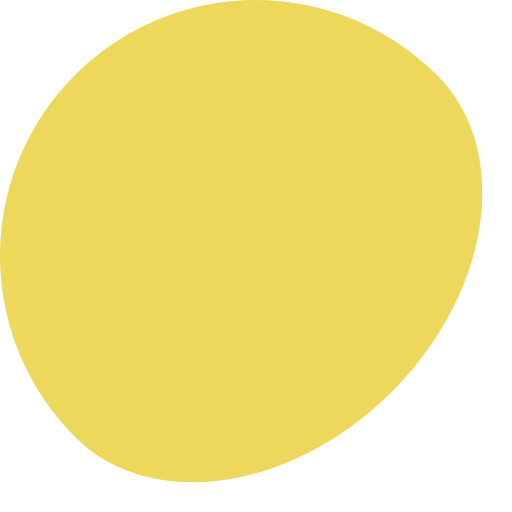
\includegraphics[scale=0.4]{planet.svg.png}

\vfill

{\Large \textsc{Altaris University Press}}

\end{center}



\pagebreak

\section{Introduction}

The present \emph{booklet} is conceived to fill a serious and sizeable void in literature on \textbf{Flavus}, the \emph{Yellow Planet}, and its inhabitants. Until now, only xenobiological and xenoanthropological research material has been available, a presentation of information very little accessible to laymen with no technical knowledge, a demographic constituting an ever growing fraction of visitors to this odd, fascinating planet.

\cmmnt{finish}

\tableofcontents

\chapter{The planet Flavus}

\section{Flavus}

Flavus is a smallish Earth-like planet orbiting a K0-class star. The common name refers to the planet's distinctly yellow tint, due to surface sulfur deposits.
%\section{Climate}

The axial tilt of Flavus is extremely modest, which leads to an imperceptible seasonal cycle and small polar circles. The temperature variation due to eccentricity of the orbit is even larger, though still minute. Therefore any given location on Flavus does not experience much difference in temperatures throughout the year.

The average surface temperature is significantly higher than on Earth. Only the polar regions, which host tropical-like climates, are inhabitable by humans. Intermediate latitudes are occupied by a vast, dry, acidic desert.

Flavus has currently very reduced tectonic activity and suffers from much more frequent asteroid impacts. The result is a relatively flat topography, mostly dominated by impact craters.

\cmmnt{picture}


\vfill
\section{The sulfur cycle}

The Yellow Planet slowly alternates between short periods of intense volcanism and long pauses of geological inactivity. During the former, copious amount of sulfur are produced, which are turned into fine dust and diluted into the sands of the planet.

When elemental sulfur concentration in sand exceeds a certain threshold, the possibility arises for a fire. Sulfur fires are awesome and terrifying, spreading quickly and then burning for days with a deep blue glow. Fires produce large columns of toxic sulfur dioxide.

The inverse direction is provided by the lifeforms native to the planet, the Plunts, which during photosynthesis consume sulfur dioxide in addition to carbon dioxide. Plunts store the absorbed sulfur in elemental form as small stones called \textbf{calculi}, which they release after their death.

At equilibrium, this feedback pair mantains a constant concentration of elemental sulfur in the sand and sulfur dioxide in the atmosphere. The latter (at ~ 10 ppm, to be compared with Earth's 1 ppm) is low enough for humans to survive, but still results in some permanently acidic rains and bodies of water.
\vfill
\pagebreak

\section{Flora}

The dominant native lifeforms of Flavus are a large class of plant-like creatures known colloquially as Plunts. Plunts perform a variant of photosynthesis in which sulfur dioxide can be also processed alongside carbon dioxide; the relevant combination of pygments (including clorophyll) gives almost all plunts a purple-blue colour.

Plunts however also possess animal-like traits; they are in fact often capable of limited locomotion and have primitive nervous-like systems. But it's the nature of their reproductive habits that is priceless for the human inhabitants of Flavus. The male organ of a Plunt consists of an elastic sac which is filled by sperm capsules over the course of a few months. When the pressure is sufficiently high, the sac bursts releasing the capsules, which are designed to be then transported by wind. The female organ instead produces an egg-like structure, a translucent white ovoid with a thick rubbery skin filled with a sugary protein syrup. The egg is topped by a receptacle, the true female organ. When a sperm capsule reaches a receptacle, a Plunt embryo is conceived and transferred to the egg.

The new individual is gestated for months inside the egg, which then hatches to reveal a cyan toadpole-like larva. The larva has some locomotive ability which it uses to get as far away as possible from the mother over the course of a few days. It then burrows the root tentacle on its head into the sand and becomes sessile, entering its adult stage.

\begin{center}
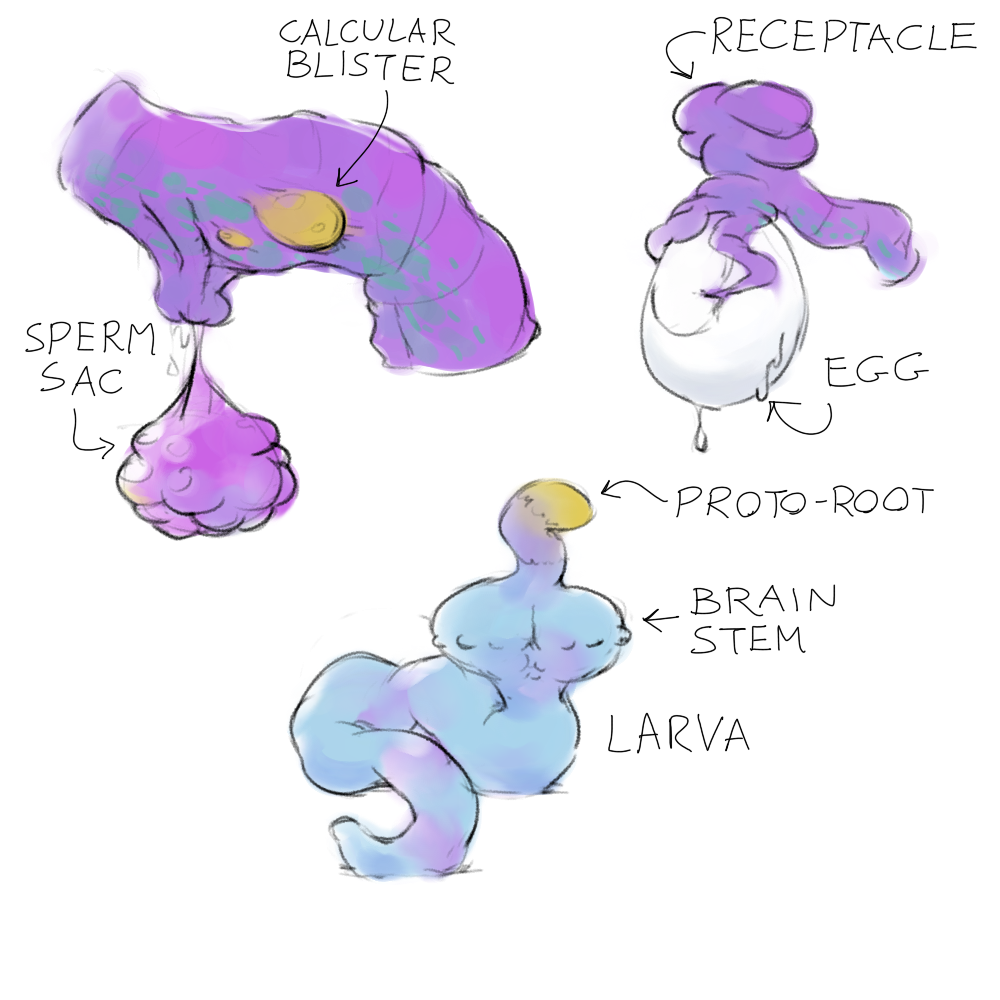
\includegraphics[scale=1.9]{../drawings/pluntorgans.png}
\end{center}

Humans eat almost exclusively unfertilized plunt eggs, since they are relatively nutrient and not toxic like most of the organs of most plunt species. Growing eggs is fairly easy, consisting essentially in sealing the receptacle so that it cannot be fertilized. Plunt eggs are more agreeable when cooked, and are slightly alcaline with an ammonia-like smell.

Plunts do not have any signficantly rigid components. They are always elastic to some extent and their trunks are analogous to the tentacles of mollusks, being kept in position (or moved) through a hydraulic system. Their gummy purple skin is covered in a watery mucus, acting as an insulant to protect them from the extreme heat. 

\vfill
\section{Fauna}

There isn't a hard-cut distinction between truly vegetal and truly animal Plunts. Some of them are distinctly animal-like, in that the photosynthetic abilities are mostly vestigial and live through consumption of other Plunts.

\cmmnt{Crab-bushes}

\cmmnt{Bluegrass}

\cmmnt{Squid birds: how they can be trained}

%\chapter{Flavan civilization}

\pagebreak

\section{Humans}

The most intelligent inhabitants on the planet are humans, or Flavans. What exactly they are doing there is unknown, and Flavans have no understanding of recollection of Earth, nor of the fact that they are not native to Flavus. Nevertheless, the planet is a harsh, inhospitable environment, with its dry, hot climate and acidic chemistry, and apparently Flavans have still not completely adapted accordingly, testifying that they haven't been around for more than a handful of millennia. Still, the small effect of these hardships on the bodies of humans are perceptible already. Flavans grow 5 to 10 cm taller than Earthlings on average as a consequence of the lower gravity, which also increases chances of bone and heart-related diseases. They have very light skin, pearly white, since UV radiation on the surface is low, owing to Flavus' star low temperature and the planet's thicker magnetic field. A darker skin tone would facilitate vitamin D deficiency and has been quickly selected against. Paradoxically, Flavus' scorching sun cannot sunburn.

The last important physiological difference is that Flavans have respiratory and digestive systems slightly more suited for acidic environments. 

Flavans live in nuclear communities (\textbf{pak}), analogous to villages and averaging 200 individuals, based in oases in the arctic regions. Frequently, travelling groups will hop between oases by crossing the desert, carrying goods, knowledge, and money.

Two main ethnic branches inhabit the Arctic. The Demorog ("square-writing") occupy the pole, the lower-left, central, and right regions, while the Bymarog ("flame-writing") live in a strip in the left. The two civilizations are connected by thin straits inbetween a row of small lakes. It makes little sense to distuinguish smaller subdivisions as Flavan cultures, by virtue of their nature, constantly mix and rearrange.

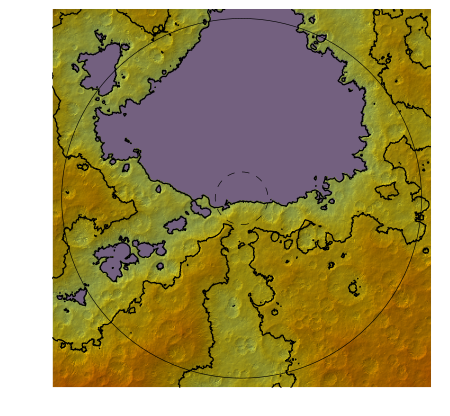
\includegraphics{../maps/map/map.png}

\cmmnt{Obviously, finish map.}

\pagebreak

\section{Fashion}

\cmmnt{copy from that reddit comment and add pics}

\pagebreak

\section{Travel, shrooms and bannering}

\begin{minipage}{0.6\textwidth}
Flavans constantly hop from village to village, for commerce, news, or to pursue a carreer; crossing the harsh desert inbetween craters is risky and dangerous however, and would requires considerable resources and skill, more than are available to the average inhabitant of this weird planet. The professional figure of the Travel Master fills this void. TMs know the polar desert intimately and are aware of all the dangers it has to offer, from the terrible heat, the ever-morphing landscape of mobile plant-like organisms and featureless topography, the constant threat of a spontaneous blue-hot sulfur fire. They are expert map-makers and map-readers, know how to keep themselves and a group of travellers alive in emergency situations, and also probably know quite a few good jokes. TM travel attire includes "sunglasses": a visor of smoked glass to see better in the bright sunlight.\\

Any village has TMs coming and going all the time; anyone who needs a ride can just contact one and pay the ticket to join the travelling group the following day. It's a good idea to check the alleged TM's credentials - their ID strip (basically a mix between an ID card, a CV, and a passport), or even checking in the Village Registry if the records match. Diving into the desert with an unskilled idiot does not end well.\\

Becoming a TM is extremely hard; it only comes after a long period of apprenticeship and the title is awarded only with the approval of four other TMs.
\end{minipage}
\hfill
\begin{minipage}{0.4\textwidth}
    \begin{center}
        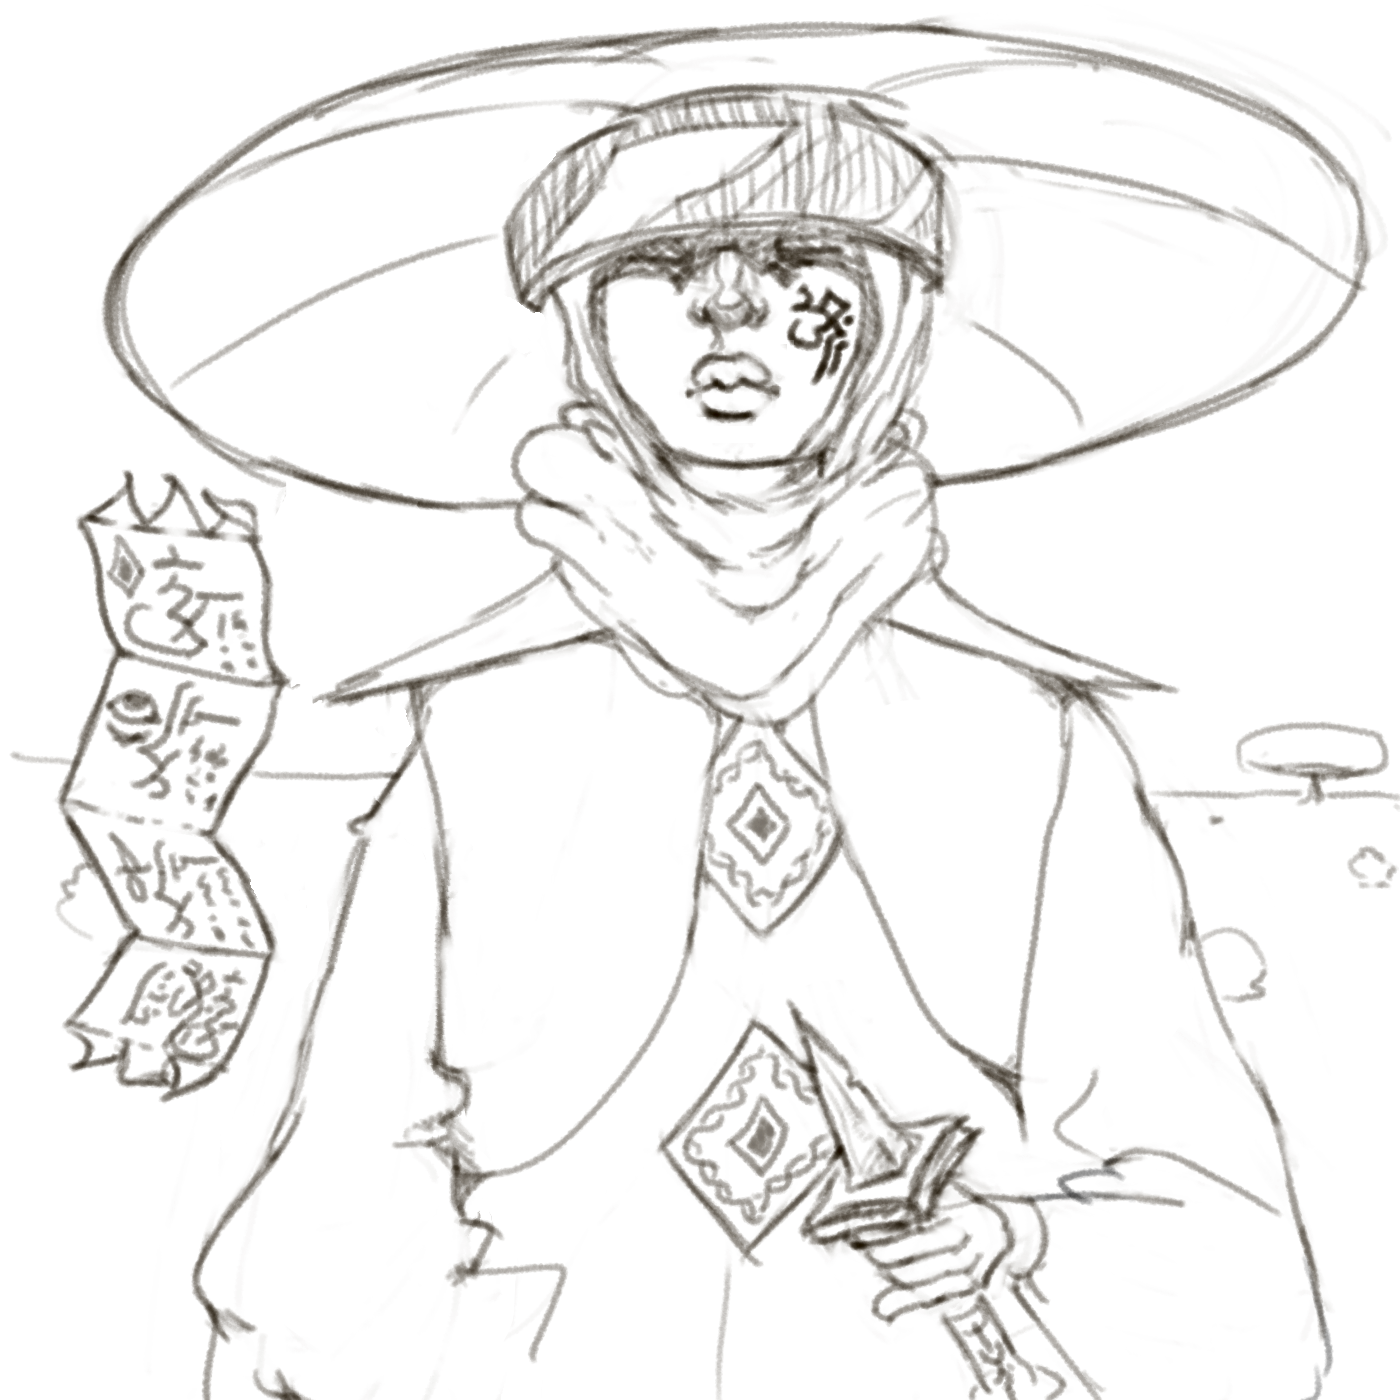
\includegraphics[scale=0.6]{../drawings/travelmaster.png}
        \captionof{figure}{a Travel Master and her ID strip}
    \end{center}
\end{minipage}

\cmmnt{add pics}

Oases are small specks in a vast, unforgiving and extraordinarily bland desert, with very few recognizable points. Even with the expertise of a TM, a traveling group walking straight into the desert in a random direction could very well walk to their death without ever sighting a village. Orientation doesn't help much, as even a small error can build up and the destination could be missed entirely. How do travelers on Flavus manage to move around consistently? The solution is provided by the single largest living beings on the planet: shrooms.

Shrooms are gigantic mushroom shaped plunts, between 100 and 200 m tall, and inhabit primarily the polar desert, avoiding the excessive humidity of the oases. They have impressive root systems, sometimes even a kilometre across, to extract the necessary nutrients for survival. The ``stalk'' is relatively thin (two to three metres in diametre) but equipped with a powerful hydraulic pump is able to sustain the weight of the very large ``cap'', actually a disc-shaped layer of branches and leaf-organs. The cap itself is very light and little dense. Shroom (and their caps in particular) are home to rich ecosystems including parasites, symbionts, and predators.

Travelers use shrooms primarily as reliable reference points. Shrooms live easily for centuries, and skilled Masters can recognize individual shrooms from the shape of the cap, even from kilometres away. Shrooms are marked on maps and named, and traveling routes "hopping" from shroom to shroom are established. Not only: even if it wasn't for orientation, shrooms still make for attractive stops for travelers: the stalk can be cut to drip out sap, which is easily filtered for drinking, and its large (although distant, considering the Sun's low altitude) shadow, where the group can rest. Sadly, they cannot literally stop in the cap's shadow and drop the tents: the shroom is so tall that the shadow moves too fast throughout the day, forcing travelers to continuously move every half-hour. Daggers used for shroom sap extraction have become a symbol of travelmastership, and TMs carry expensive personal dagger with elaborate designs.

Upon passing by an undiscovered shroom, the Master will mark it with a banner of their village (or occasionally one of the recently visited villages), a flag-like piece of cloth bearing the pak name. These banner are manufactured in advance by children in the pak and travelers always carry a few. The banner has a pouch in which travelers insert "update documents": writings reporting on their travel, maps, news on the recently visited villages, general updates, and a bit of gratuitous personal diary. The next visitors to the shrooms can then enjoy this information and add their own to the shroom's archive. Travelers communicate much more information through bannering than through actually meeting in travel, which happens rarely.

\cmmnt{I have this drawing already; where the hell did I put it?}

A shroom banner for the Ramy village, with embroidery in geometric style. Below the word *ramy* itself, the map symbol for a village is used as a shorthand for pak. On the bottom, a pouch for update documents.

\pagebreak

\section{Villages}

\cmmnt{write everything, copy from reddit cmmnt}


\includegraphics{../drawings/bigseal_gold}

\cmmnt{also copy caption for this}


\pagebreak

\section{Sex, Gender and Parenthood}

Flavans don't like children. Even in what is relatively speaking an oasis, the harsh lifestyle makes survival of the community the first preoccupation; procreation, and thus a noticeable population increase in a small village is seen as damaging. Bearing child is therefore heavily regulated and the mother is required to pay the *pak* authority a fee whose value is regularly updated depending on the village's situation. Failure to produce the money can result in expulsion.

This "demographic phobia" has its origin in Flavan folklore of villages destroyed by overpopulation, and results in very unusual ideas on sex drive, reproduction, gender, and the role of children in society. Children are perceived as "impure", "indecent" or more precisely "unstructured"; physician Baryk-t Ardeman describes the process of growing a child into an adult as akin to the drying of gum-birch skin, removing its toxic "blue" essence to reveal a structured individual:

*the child is born as an amalgalm of the elements, imbibued with blue as the skin of the gum-birch. Living amongst the yellow, it is dried, and the blue drips, and it takes face.*

The genitals and nose of children are always to be covered in public, and the distinction between child and adult is stronger than even that between male and female, a feature reflected in the Flavan language. A child is grown and educated by his mother only; there is no concept of fatherhood on Flavus. The biological father has no responsibilities nor rights concerning the child. The closest idea to fatherhood is a form of tutorage in which an adult (almost always male) trains a child in various skills, most importantly reading and writing and the basic of travelling; it's not uncommon for an emotional bond to develop, nor is it frowned upon. A child can have any number of tutors.

Children become adults as they reach ... Visits (... Earth years) of age, at which point they are "uncovered" in a ceremony. To emphasize that the adult Flavan is not far from being considered a distinct person from themselves as a child, adults count their age starting from their uncovering.

Because reproduction is almost always seen in such a negative light, Flavans rationalize the sex drive as "intrinsic suffering" to being alive, and in alignment with their philosophy believe that like all forms of pain it should be embraced and redirected towards good or constructive purposes. Therefore, they understand the need for recreational sex. There is variety in the sexual habits of Flavans, but an obvious constraint is that vaginal penetration is forbidden (unless the woman is prepared to have - and pay for - a child). Demorog do not really perceive any difference between male and female and tend to engage in often short, vaguely monogamous relationships, either heterosexual or homosexual. Bymarog forbid all recreational heterosexual contact, but gladly accept homosexual (male and female) pairings, but do not have any concept of relationship or commitment at all.

The body of a Flavan is considered their most prized possession, because of the suffering associated with owning it. (In fact, the female body is regarded as even more valuable, because of the menstrual cycle and the associated physical pain and discomfort). Therefore, Flavans classify rape as a form of theft, which is an unforgivable sin. All forms of rape are punished with expulsion, in addition to the child fee in case the rape results in a pregnancy.

The reason for reduced gender differences in Flavan society is mostly that there is neither much hunting, nor child-bearing to do on Flavus. (Side note: Flavans would not be able to understand an arrow symbol). Gathering, building and travelling require skills common to both sexes and almost all roles in Flavan society include men and women in comparable fractions. Flavan grammar does not distinguish male and female, and while most proper names are indeed gendered, a good portion of them are Unisex. In fact, the very physician quoted above, Ardeman of the Baryk village, bears such a name and it's not possible from their writing to infer whether they were a man or a woman.

\pagebreak

\section{Culture}

%When they laugh, Flavans take out their tongue and keep it between their teeth.

\cmmnt{Perhaps section about behaviour, politeness, hospitality, conflict resolution}

\pagebreak

\section{Science}

\cmmnt{The School, education, teaching and research}

\pagebreak

\section{Astronomy and Religion}

In addition to the fixed stars, the only two astronomical objects that the Flavans are aware of are the Star and the Wanderer (Vulcan being too close to the Star to be visible). Flavans believe these two objects to be identified with \cmmnt{copy that nice idea about the pantheon}

The Wanderer is a bright, spectacular sight when in opposition, that is when it is closest to Flavus, and reaches maximum altitude at midnight. In fact, Flavans measure years as spanning between consecutive oppositions (which they call "visits") of the Wanderer, instead of through the motion of their sun on the fixed stars as it is done on Earth. Thus, Flavans prefer the synodic period of the Wanderer with respect to Flavus, rather than Flavus' own sidereal period, to act as a measure of time. This choice is coherent both with the absence of detectable seasons and with the secondary role the "fixed" stars have in Flavan cosmology.

\cmmnt{finish finish finish}

\cmmnt{add main religion}

\pagebreak

\section{Food}

\cmmnt{pics!}

\cmmnt{Recipe for dhlorg}

\vfill

\section{Magic and Medicine}

\cmmnt{Chirocasting, fever, bloodletting, humoural theory}


\newpage
\section{Writing}

Flavan writing arises from the practical need of mapmaking. Since mutual intelligibility is key, Flavans essentially all use one unified script, but with distinct styles of rendering shapes. The Flavan script was originally an alphabet (with consonant and vowels being represented by distinct glyphs) but has transitioned into an abugida as consonant and vowel glyphs have fused into new forms. It is written vertically, more precisely top-to-bottom, right-to-left; words within a single column are separated by a dot. The script is specified in detail in chapter \ref{script}.

The most bizzarre aspect is the writing tool Flavans use, the pen-leech. Pen-leeches are parasitic worm-like animals distributed throughout the Polar regions, and which feed on large plunts, in particular shrooms. The pen-leech attaches to the trunk of the plunt through its two cartilage fangs; when secured to the skin it squeezes out a corrosive mucus, essentially digesting the host externally, then sucks back the mucus into its body for absorption. This cycle is repeated. Pen-leeches are barely taxing on the gigantic shrooms and the latter can often host hundreds or thousand of parasites with no real damage to itself. Flavans exploit the leeches' sucking and splurting ability to use them as pens. Travellers collect a few as they hop by a shroom. Once brought home to the village, they are prepared as such:

\begin{itemize}
\item The brain node, in the posterior of the creature, is cut off alongside the vestigial root. This kills the leech :(
\item The carthilage fangs are removed carefully to retain a smooth, circular mouth.
\item The leech is cleaned and hanged to dry out the sap
\end{itemize}

\cmmnt{add drawing}

The pen-leech, now more rigid and elastic, is then ready to be used similarly to a fountain pen, sucking in an ink produced from ashes, and releasing it on paper when squeezed. This gives rise to the characteristic roundish strokes in Flavan writing. Pen leeches do not last more than a month before starting to rot, and thus must be replaced frequently - therefore, there is no such thing as a "luxury" pen-leech, even though a skilled pen-leech preparer is highly regarded.

\cmmnt{v this could be moved to script chapter.}

Writing styles can be split roughly into three general categories:

\begin{itemize}
\item The Demorog "geometric" style, mostly employed in embroidered or chiseled designs or in very large writings (such as on walls). Occasionally also used in tattoos and maps.
\item The Demorog "cursive" style, for maps, letters, books, and everything in pen-leech.
\item The Bymarog "flame" style
\end{itemize}

Here are the words *Demorog* (right) and *Bymarog* (left) themselves, written respectively in geometric, cursive, and flame style.

The words denoting the two ethnic groups themselves (Demorog = square-writing, Bymarog = flame-writing) refer to the appearance of these writing styles.

A few designs for the word *moshl* ("mother")

\cmmnt{add pic\ldots}

\pagebreak

\section{Tattoos and makeup}

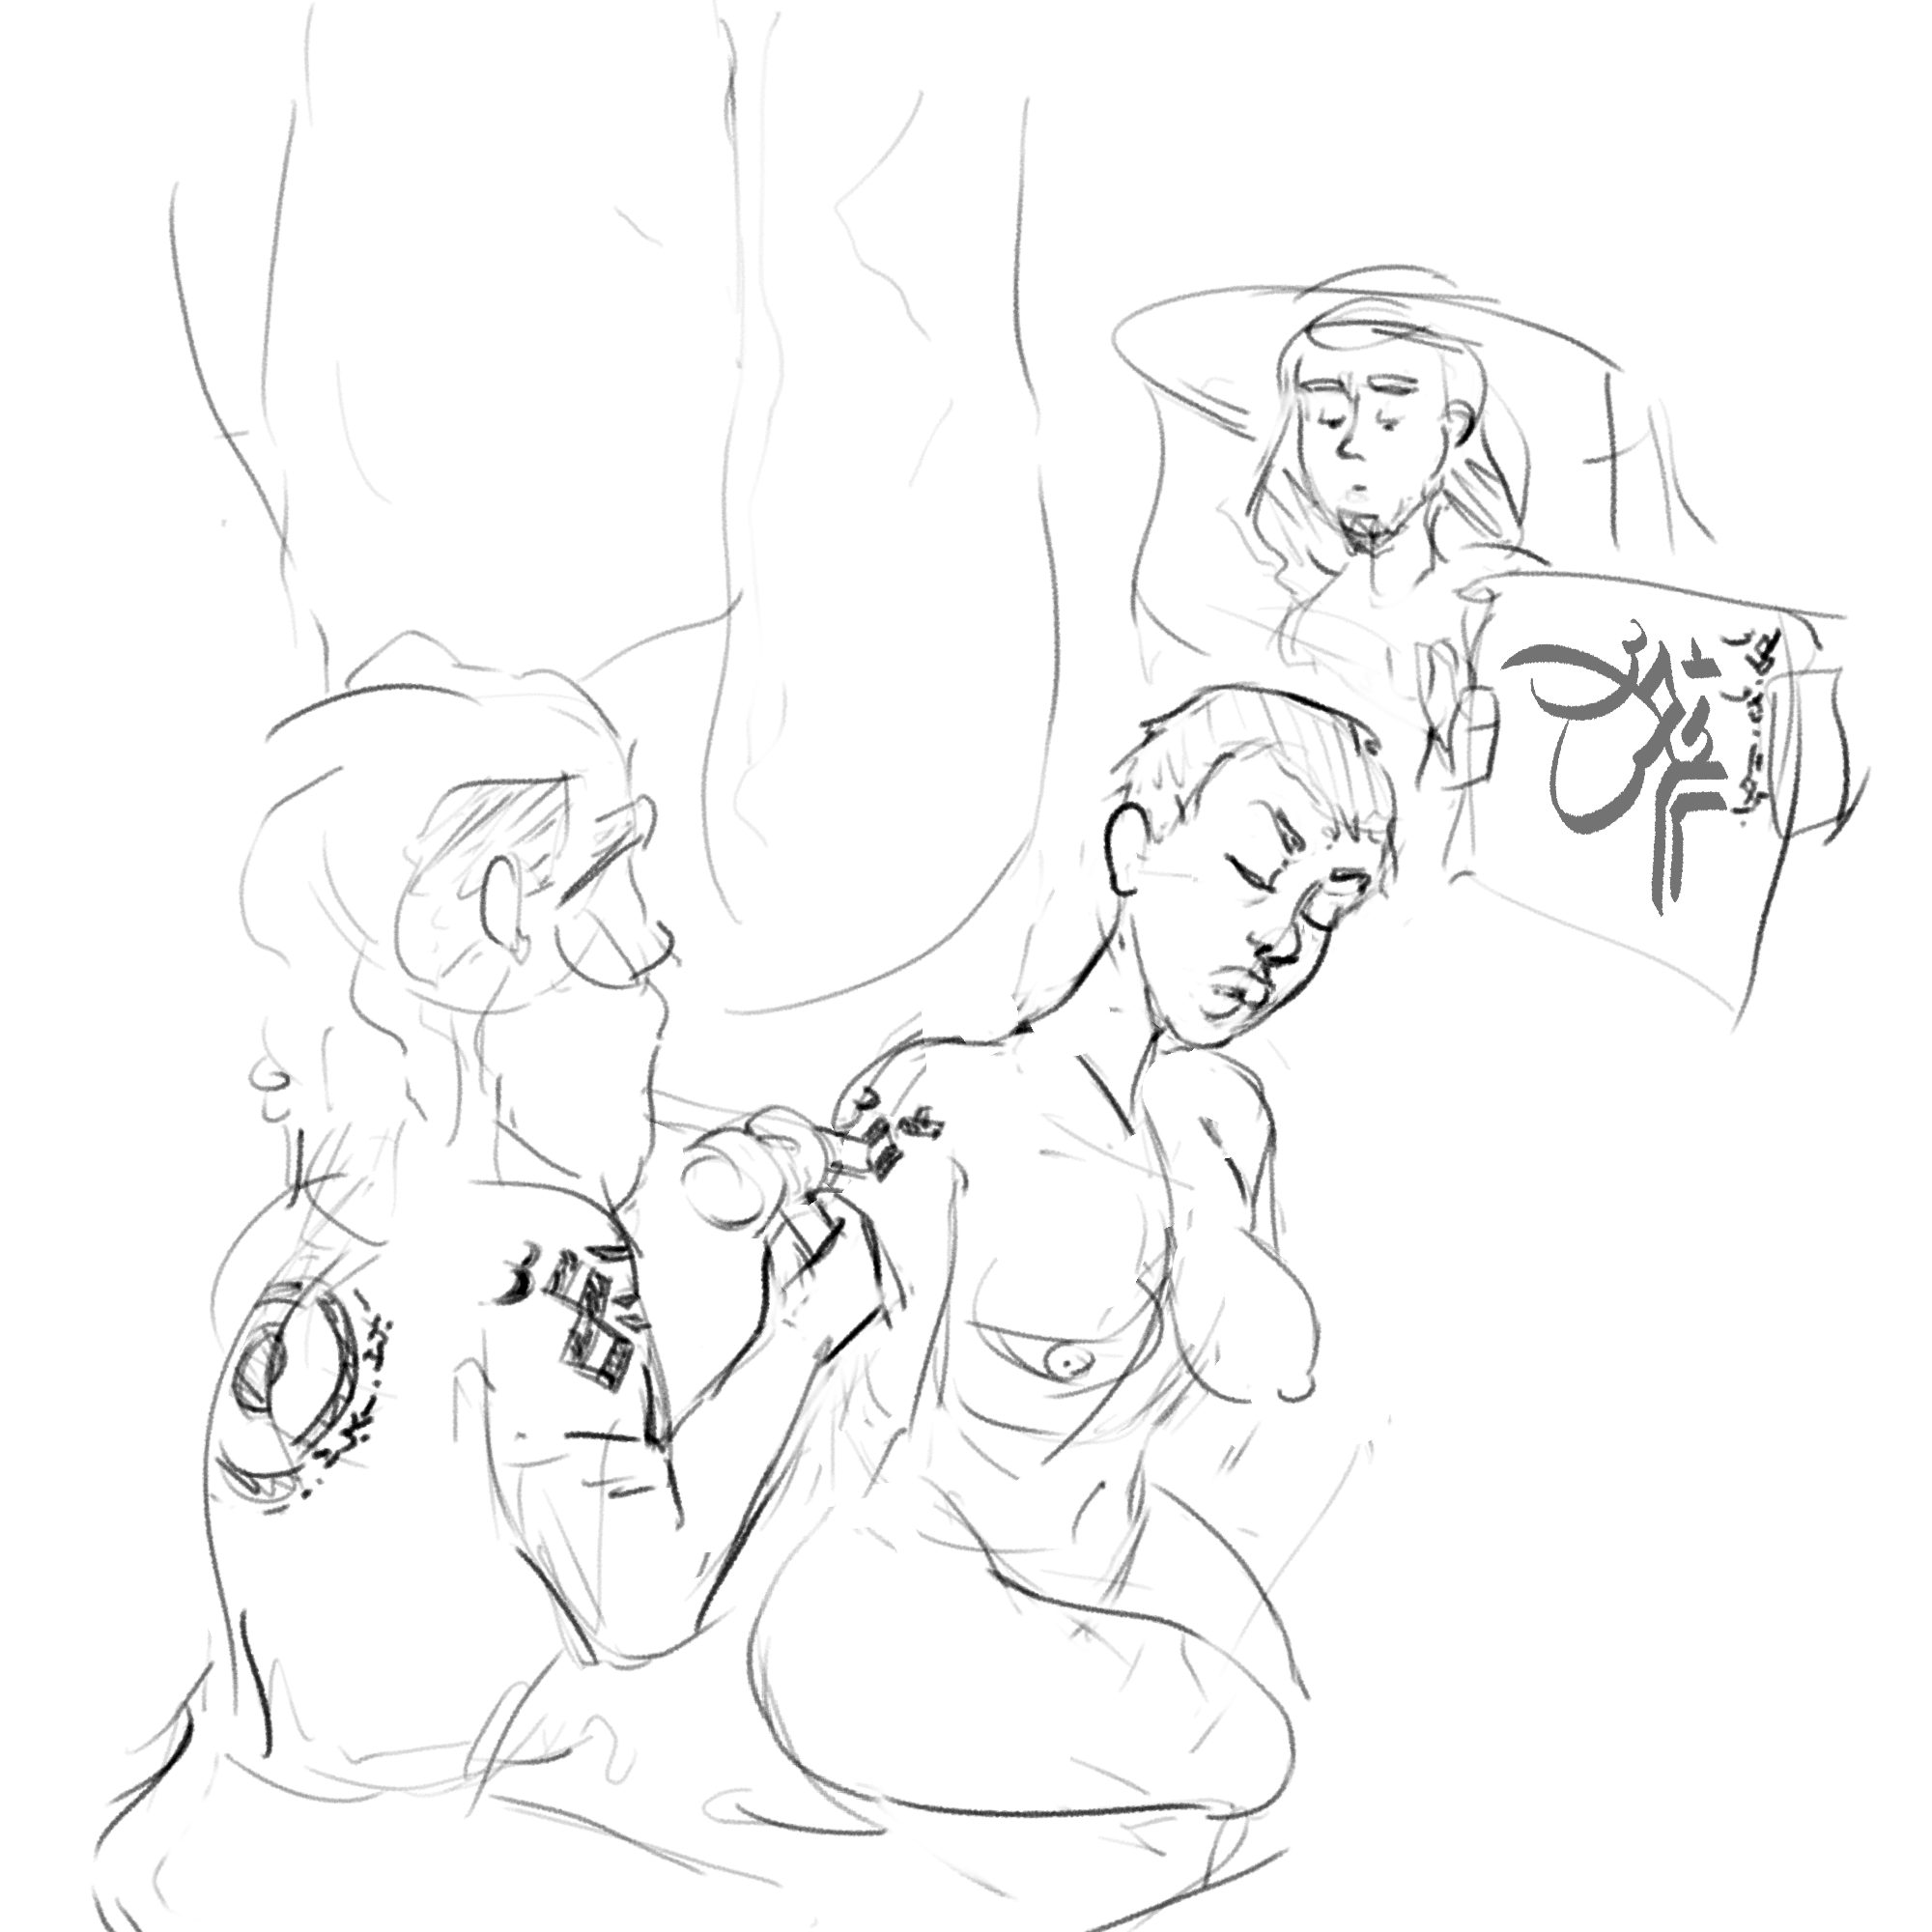
\includegraphics{../drawings/tattoo.png}
\cmmnt{finish drawing ofc.}


\cmmnt{and write everything:
    \begin{itemize}
        \item Name tattoos\\
        \item Chiroportals\\
        \item Graduation eyebags
    \end{itemize}
}

\pagebreak

\section{Colours}
\cmmnt{Leave here or move to lang chap? Add phylosophical repercussions}





\begin{tabu}{c l c}

	\crekt[white]	& \rdelim]{1}{3mm}[White] &\\
\crekt[yellow] &  \rdelim]{3}{3mm}[``Yellow''] &\\
\crekt[orange] & &\\
\crekt[red]	& &\\
\crekt[magenta]	& \rdelim]{4}{3mm}[``Blue''] &\\
\crekt[purple] & &\\
\crekt[blue] & & \\
\crekt[cyan] & & \\
\crekt[green] &  \rdelim]{2}{3mm}[``Green''] &\\
\crekt[gray] & & \\
\crekt[black] &  \rdelim]{1}{3mm}[``Black''] & \\

\end{tabu}

\pagebreak

\section{Music}

Flavan music is strongly percussive and often based on a specific 5/4 rhythm:

\begin{abc}[name=rhythm]
X: 1 % start of header
K: C % scale: C major
M: 5/4
c3 c3 c2c2  |
\end{abc}

%\begin{abc}
%X:4
%T:Cronin’s Hornpipe
%R:hornpipe
%S:Keenan and Glackin
%E:7
%M:C|
%L:1/8
%K:G
%BA|GABc dBde|gage dega|bage dBGB|cABG A2BA|!
%GABc dBde|gage dega|bage dBAB|G2G2 G2:|!
%fg|afd^c d2ga|bged e2ga|(3bag  (3agf gedB|(3cBA AG AcBA|!
%GABc dBde|~g3e dega|bage dBAB|G2G2 G2:|!
%\end{abc}
%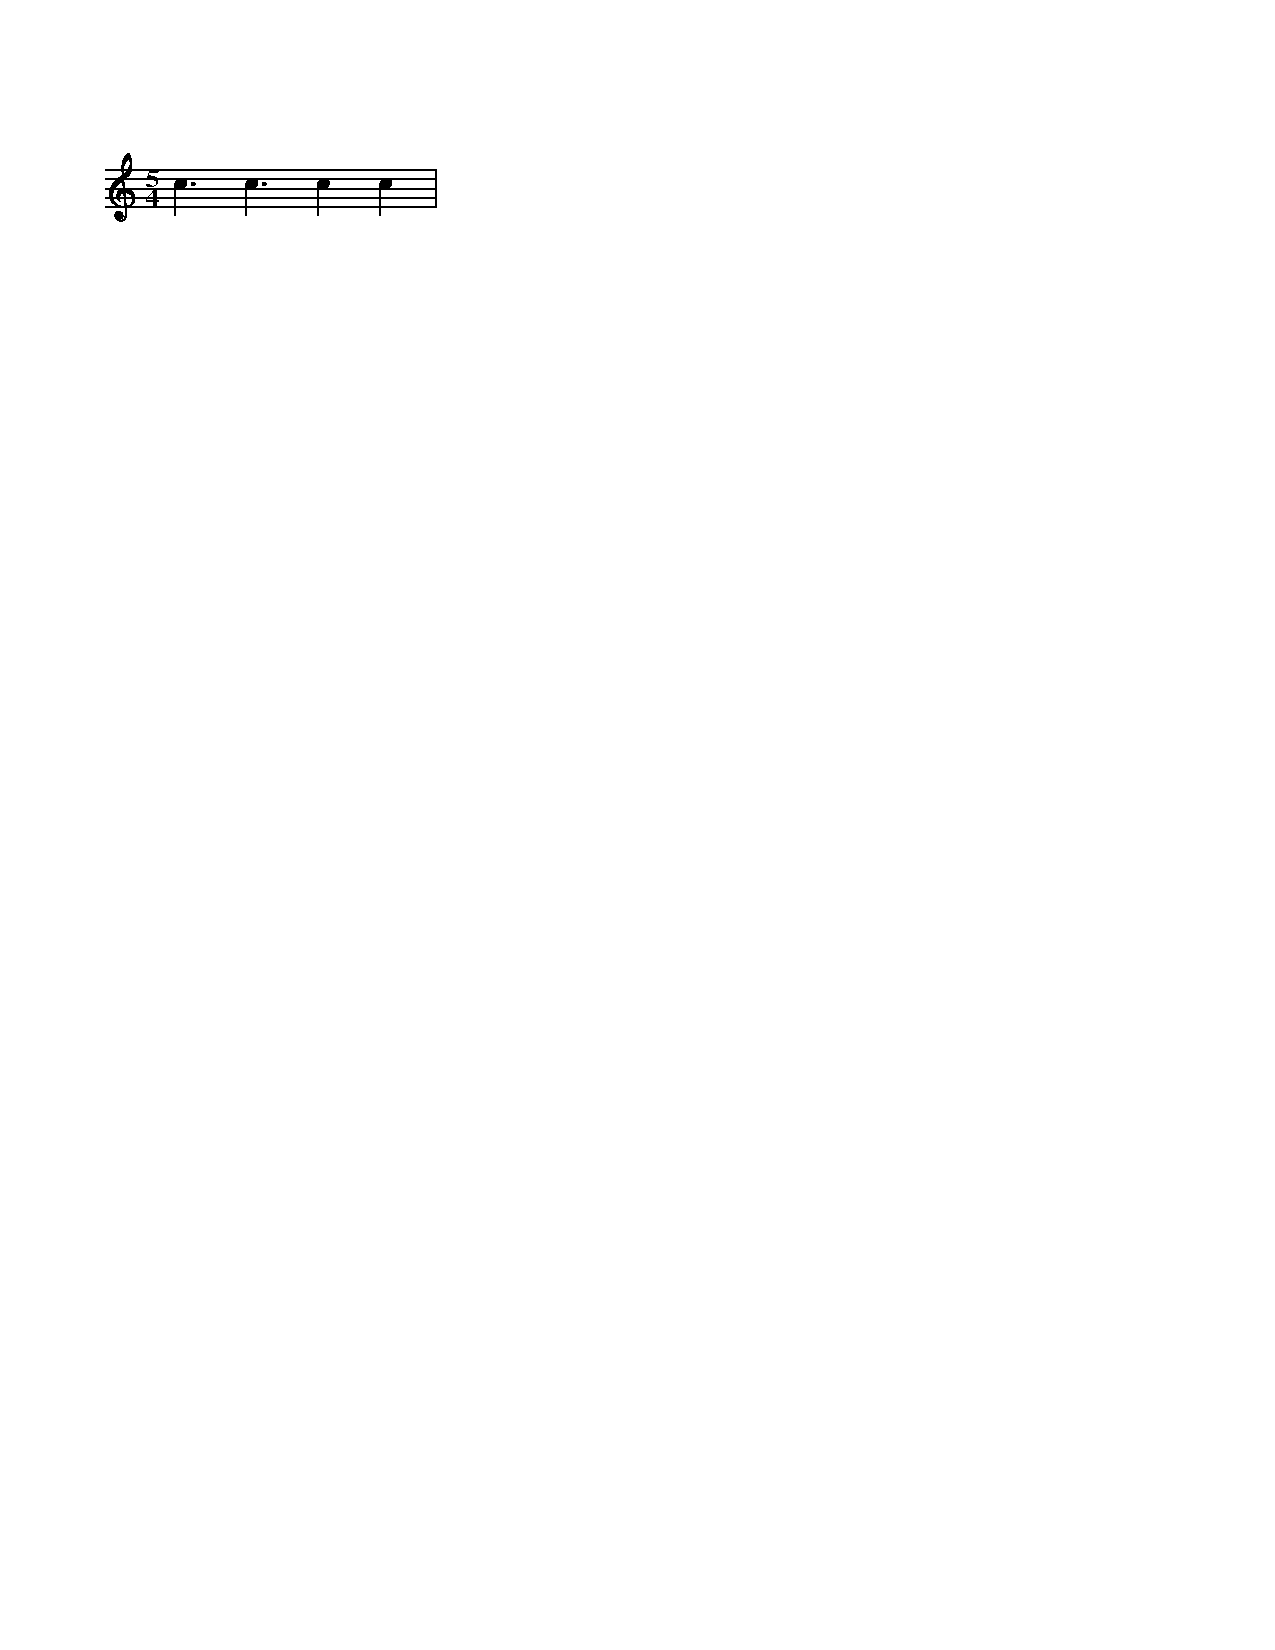
\includegraphics{rhythm}

And melodies are played in a hexatonic scale:

\begin{abc}[name=scale]
X: 1 % start of header
K: G 
L: 1/4
M: 5/4
CDEFGA|c
\end{abc}

%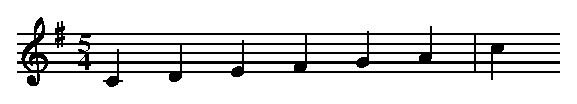
\includegraphics{scale}

(This representation in terms of equal temperament notes is of course an approximation). This scale can be seen as an extension of the major pentatonic to include the maximally dissonant flat fifth / sharp fourth, or equivalently as a subset of the western lydian scale. The inclusion of the tritone interval, a modern and daring device which on Earth had essentially never been truly appreciated as anything else than \emph{diabolic} before Romanticism, is baffling - the other intervals are instead extremely natural and based on small integer ratios. (Arguably, the pentatonic scale is likely universal to all humans). 

Music is played by traveling "bands" composed of a Drummer, a Lead vocalist, and one or two Backing vocalists. Songs take a vaguely choral form as the backing vocalist open by singing the title/refrain in a constant note; this works as an "introduction" to the piece of music, and also establishes the fundamental note and the tempo. The Drummer joins in and the Backing continues to hum the refrain on the fundamental. After, the Lead introduces the main melody and lyrics, harmonizing on the backing's drone. Flavan music is thus essentially biphonic, though the bass is simply a drone, very rarely changing. Lyrics almost always tell a story, either humorous (and vulgar) or tragic, and the refrain itself is very often an ironic twist on the subject that is only understood after the main lyrics are presented, even though it gets continuously repeated throughout the song. Sometimes, the refrain even rhymes with the last verse of the lyrics.

A translated Demorog example:


\textbf{It's empty like death}

\begin{verse}
\emph{(backing starts droning: ``it's empty like death'')}

Abar of the Shefe village has\\
brimstone hair and silver sweatdrops\\
Rkon of the Bybang village wants\\
the sweet green breasts\\
that Abar of the Shefe village has.

\end{verse}

\begin{verse}

But everytime that Rkon comes\\
to Shefe village and Abar's tent\\
Abar's mother is always there.

\end{verse}

\begin{verse}



Abar writes a letter then,\\
``come to visit in seven days,\\
and no one will be in the tent.''\\
\end{verse}

\begin{verse}


Rkon of the Bybang village reads,\\
Rkon walks from here to there\\
sulfur feet he has to have\\
He enters Abar's tent and


\emph{(it's empty like death)}

\end{verse}

In this interesting example, the refrain is doubly deceiving as it also sets up a dramatic mood which is then inverted by the humorous subject. The expression "empty like death" refers to the fact that the internal organs of dead plunts decay much faster than their skin, which leaves them with a "deflated balloon" appearance. The curious combination "green breasts" makes sense in the context of Flavan perception of colour, and probably refers to a grayish-pinkish hue of very pale skin.



\pagebreak

\section{Psychedelics}

\cmmnt{do}


\chapter{The Flavan Language}
{\Large Reference Grammar and Lexicon}

\vfill
\vspace{-30pt}
\begin{center}
    {\fontsize{100}{80}\selectfont \flav{n ongok keb}} 

    \emph{``If I could speak light...''}
\end{center}
\vfill

\pagebreak

\section{Introduction}

The language that Flavans speak in does not seem to have any discernible relationship with any ever spoken on Earth. It is thought therefore that most of the basic structure of the Flavan language has indipendently developed on the planet. As a result, it includes a combination of alien and unfamiliar constructions and more usual features that might have the character of linguistic universals of all humans. It is hard however to make this kind of generalizing statements with confidence since Flavus has likely only ever hosted \textbf{one language} at any given time: the constant rearrangement of population, and an army of travelling merchants perennially jumping from village to village, has guaranteed that differences in all aspects of culture, language in particular, are smoothed out and always remain somewhat modest. Thus Flavan enjoys limited regional variations, almost entirely in pronunciation, and remains mutually intelligible from the left-most of Bymarog villages to the antipodal dialect of the Demorog settlements in the far-right.

As per the origins of this language, little is known about Flavans in general before around 1500 years ago. Villages at this time likely only occupied a smaller area in the central region, and the small population used a strongly agglutinative language which is known as \textbf{classical Flavan}, written in a rune-like alphabetic script meant for carving. Classical Flavan's pronunciation is unknown but has been tentatively reconstructed as having the unusual four-vowel inventory \ipa{a e o 1}.

Between 900 and 800 years ago the population increased dramatically as technological advances allowed Flavans to explore and colonize the entire survivable Northern cap, resulting in the branching of the Bymarog\footnote{the name \textbf{bymarog} (flame-writer) is used here anacronistically, since the modern script has not been introduced yet at this point.} culture in the somewhat isolated left region. It's only after the opening of the School of Karobet, which introduced new writing tools and the \textbf{modern Flavan script}, an abugida, that one begins to find an immense amount of written documents, most importantly maps and village registries, which testify that strong changes have already begun in the spoken language, mostly moving it into slightly fusional territory.

In the remaining years, Flavan has evolved significantly in syntax/grammar (developing a very strict word order for example) and phonology (the Classical Flavan phoneme \ipa{1} was unstable and underwent fragmentation into significantly different sounds in the various dialects). The cultural and linguistic divide between \textbf{Demorog} (``square-writers'') and \textbf{Bymarog} (``flame-writers'') was born. However, the aforementioned continuous cross-cultural contact has kept Flavan relatively very similar to itself as it changed in time. The current situation is known as \textbf{Modern Flavan}, and is the language this chapter will try to introduce.

Every respectable reference grammar on a language should at least present the language's own name for itself before anything else; however, this is simply impossible in our case: Flavans know one culture, with one language, and one script - granted, with modest variations in customs, manner of speaking, and writing styles. They do not conceive of a boundary between themselves and an outside - they don't need a word to mark this border. Therefore, there is no Flavan word for \emph{the Flavan language}, or \emph{the Flavan people}. To them, it's just speaking, and just people.

\pagebreak

\section{Phonology and phonotactics}

The phonetic inventory of Flavan is most conveniently presented by means of their own organization in terms of an ``alphabet'', which is a list of allowable consonant clusters and single vowels. Curiosly, they arbitrarily separate consonantal sounds into ``common'' and ``uncommon'', crudely reflecting the frequency of those phonemes in spoken language. The following chart lists the Flavan names for the phonemes, their average Demorog and Bymarog pronunciations, their romanization, and also introduces the corresponding glyphs in the Flavan abugida, which will be better explained later.

%\begin{multicols}{2}

\begin{adjustbox}{center}
{\large
    \begin{tabu}{c >{\bfseries}c c c >{\bfseries}c }
	\multicolumn{5}{c}{The ``Males'' (common consonant clusters)}\\
	\rowfont{\small}
    Glyph & \nf{Rom.} & \multicolumn{2}{c}{Pron. (Dem./Bym.)} & \nf{Name} \\
	\hline 
    \flav{-}	& \nf{None}	& //\footnotemark		& \apa{}		& pode\\
	\flav{m}	& m	& \ipa{m}	& \apa{m}	& ma \\ 
	\flav{p}	& p	& /p/		& \apa{p}		& pa\\
	\flav{b}	& b	& /b/		& \apa{b}		& ba \\
	\flav{n}	& n	& \ipa{n}	& \apa{n}	& na \\ 
	\flav{t}	& t	& /t/		& \apa{t}		& ta\\
	\flav{d}	& d	& /d/		& \apa{d}		& da\\
	\flav{ng}	& ng	& \ipa{N}	& \apa{N}	& nga \\ 
	\flav{tt}	& tt	& \ipa{t:}	& \apa{t:}	& kotta\\
	\flav{dd}	& dd	& \ipa{d:}	& \apa{d:}	& kodda\\
	\flav{shl}	& shl	& /\textesh l/	& [\c{c}l]	& shla\\
    \flav{k}	& k	& \ipa{k} (or \apa{x})	& \apa{P}	& ka\\
	\flav{g}	& g	& \ipa{g}	& \apa{g}	& garyn\\
	\flav{dh}	& dh	& \ipa{D}	& \apa{z}	& dhe \\
	\flav{dhl}	& dhl	& \ipa{Dl}	& \apa{zl}	& dhla \\
	\flav{s}	& s	& \ipa{s}	& \apa{s}	& syk \\
	\flav{sh}	& sh	& \ipa{S}	& \apa{\c{c}}	& shyk \\
	\flav{f}	& f	& \ipa{f} (or \apa{v}) & \apa{v} & fa\\
\flav{r}	& r	& \ipa{r}	& \apa{l} & ra \\
\flav{rd}	& rd	& \ipa{rd}	& \apa{rd}	&rda \\
\flav{rk}	& rk	& \ipa{rk}	& \apa{rk}	&rka \\
\flav{rb}	& rb	& \ipa{rb}	& \apa{rb}	&rba \\
\end{tabu}
\begin{tabu}{c >{\bfseries}c c c >{\bfseries}c}

	\multicolumn{5}{c}{The ``Females'' (rare consonant clusters)}\\
	\rowfont{\small}
    Glyph & \nf{Rom.} & \multicolumn{2}{c}{Pron. (Dem./Bym.)} & \nf{Name} \\
	\hline 
	\flav{bl}	& bl	& \ipa{bl}	& \apa{bl}	& bla \\
\flav{ttf}	& ttf	& \ipa{t:f}	& \apa{t:f}	& kottfa \\
\flav{ttl}	& ttl	& \ipa{t:l}	& \apa{t:l}	& kottla \\
\flav{ttk}	& ttk	& \ipa{t:k}	& \apa{t:P}	& kottka \\
\flav{ttg}	& ttg	& \ipa{t:g}	& \apa{t:g}	& kottga \\
\flav{rg}	& rg	& \ipa{rg}	& \apa{rg}	& rga \\
\flav{sg}	& sg	& \ipa{zg} (or \apa{Dg})	& \apa{zg}	& zga \\
\flav{gm}	& gm	& \ipa{gm}	& \apa{gm}	& agme \\
\flav{rm}	& rm	& \ipa{rm}	& \apa{lm}	& rma \\
\flav{pd}	& pd	& \ipa{pd}	& \apa{pd}	& pda \\
        	
		\hline\hline
		\multicolumn{5}{c}{The ``Children'': Vowels}\\
		\rowfont{\small}
        Glyph & \nf{Rom.} & \multicolumn{2}{c}{Pron. (Dem./Bym.)} & \nf{Name} \\
		\hline 
None		& a	& \ipa{a}	& \apa{a}	& atta\\
\flav{e}	& e	& \ipa{e} (or \apa{E})	& \apa{e} (or \apa{i}) 	& etta\\
\flav{y}	& y	& \ipa{1} (or \apa{i}, \apa{W})	& \apa{u}, \apa{y} & ytta \\
\flav{o}	& o	& \ipa{o} (or \apa{O})	& \apa{O} & ordar\\

    & & \multicolumn{2}{c}{(see section \ref{ytta})} &  




\end{tabu}
}
%\end{multicols}
\end{adjustbox}

\footnotetext{The \textbf{pode} (//) is not an actual phoneme, but simply a vowel carrier necessary to represent a vowel without a preceding cluster in the Flavan script.}

A Flavan word has a fairly rigid structure. It must alternate consonantal (K) and vocalic (W) units, so for example W, KW, WK, KWK, KWKW are allowed words. A consonantal unit is strictly one of the aforementioned clusters, while W is either one or (less commonly) two vowels (whether this results one or two sillables depends on diphthongization, explained later). All consonant clusters can appear in any position.

A few words are composed of a single consonant. These are \textbf{n} \apa{\s{n}}, \textbf{m} \apa{\s{m}}.

%A flavan word is just an alternating sequence of consonant clusters and vowels (with at least one vowel). So, if C is a cluster and V is a vowel, words can be V, CV, VC, CVC, VCV, CVCV, \emph{etc}. Any clusters can be at the beginning, middle or end of a word.
%
%It is occasionally possible for two vowels to be consecutive (VV) as a consequence of affixing. In that case, if the vowels are different they form a diphthong.

As a final note, it is possible for the cluster \ipa{kt} (actually pronounced \apa{xt}) to appear exclusively in word-final position. This is not understood by Flavans as a distinct ``letter'' as it arises from a vowel elision in some genitive suffixes. Notation for \ipa{kt} is explained in the section for the script.

\subsection{Pronunciation rules I}

\begin{itemize}
    \item \textbf{hard shyk:} waord-initial \ipa{S} followed by a vowel is pronounced \apa{\t{tS}}. Example: \textbf{sho} \flav{sho} \apa{\t{tS}O}, \emph{we (inclusive ergative)}
    \item \textbf{ytta assimilation:} when not before another vowel, \ipa{1r}, \ipa{1m}, \ipa{1n} become a syllabic consonant \apa{\s{r}}, \apa{\s{m}}, \apa{\s{n}}. Example: \textbf{yrk} \flav{yrk} \ipa{\s{r}k}, \emph{and},  \textbf{kym} \ipa{k\s{m}}, \emph{while}. Some speaker also assimilate \ipa{1N} \textrightarrow \apa{\s{N}}, but this is fairly rare. Assimilation does not happen if the \textbf{y} is preceded by the same consonant that would become syllabic; e.g. \textbf{ryrga} \flav{ryrga} \ipa{"r1rga}, \cmmnt{meaning}, and not \ipa{"r\s{r}ga}.
    \item \textbf{mid opening:} \ipa{e} and \ipa{o} when stressed open up to \apa{E} and \apa{O} respectively. Example: \textbf{rgodha} \flav{rgodha} \ipa{"rgO.dh:a}, \emph{long}, and \textbf{egord} \ipa{"Egord}, \emph{examination}
    \item \textbf{syllabic l:} word-final \ipa{l} after a consonant becomes syllabic \apa{\s{l}} (this creates a new syllable). Example: \textbf{moshl} \flav{moshl} \ipa{"mO.S\s{l}}, \emph{mother}. (Some speakers do the same with word-final \ipa{gm} to make it \apa{g\s{m}}, others insert a schwa: \apa{gm@}).
    \item \textbf{nasalization:} (rule not always applied) a vowel\footnote{Actually, the syllabics could in principle also nasalise, however two of them are already nasal and \apa{\s{l}} cannot appear after \apa{N}. The only remaining one is \apa{\s{r}}, which following \apa{N} becomes the nasal syllabic trill \apa{\~{\s{r}}}. This very rare sound only appears in a few words, including \textbf{nyngyr} \apa{"njW.N\~{\s{r}}}, \emph{sweat}. } following \ipa{N} will become nasal. Example: \textbf{ngon} \flav{ngon} \ipa{N\~on}, \emph{I (ergative)}
    \item word-final \ipa{D}, or \ipa{D} between two vowels becomes geminated: \apa{D:}. Example: \textbf{my agaredh} \flav{my\\agaredh} \ipa{mj1aga'rED:} \emph{goodbye}
    \item \ipa{r} alone between two vowels with at least the first unstressed becomes a flap: \apa{R}. Example: \textbf{pottarat} \flav{pottarat} \ipa{pot:a'Rat}, \emph{sew}.
    \item \textbf{diphthongization:} some pairs of vowels when adjacent, even between different words, will be pronounced as a single sillable, either a diphthong or a vowel + semivowel pair. We will call both of these cases a ``diphthong'' employing a common misnomer. The diphthongs and their pronunciations are as follows:

\bgroup
\def\arraystretch{1.5}
\begin{center}
    \begin{tabular}[]{|>{\bfseries}c | c | c|}
        \hline
        {\normalfont Pair} & Unstressed & Stressed \\\hline \hline
        ae & \apa{\t*{ae}} & \apa{\t*{aE}} \\
        ao & \apa{\t*{ao}} & \apa{\t*{aO}} \\
        ea & \apa{\t*{ea}} & \apa{\t*{Ea}} \\
        eo & \apa{\t*{eo}} & \apa{\t*{EO}} \\
        ey & \apa{@} & \apa{\t*{EW}}\\
        oa & \apa{wa} & \apa{\t*{Oa}} \\
        oe & \apa{we} & \apa{\t*{OE}} \\
        ya & \apa{ja} & \apa{\t*{Wa}} \\
        ye & \apa{je} & \apa{\t*{WE}} \\
        yo & \apa{jo} & \apa{\t*{iO}}\\\hline
    \end{tabular}
\end{center}
\egroup

All other pairs (e.g. \textbf{ay} or \textbf{oo}) either never appear in Flavan or if they do, they do not diphthongize and are pronounced as two separate syllables. Note that this rule is applied \emph{after} ytta assimilation, for example \textbf{babe yrk} is \apa{"ba.be \s{r}k}, not \apa{"ba.b@rk}.

\end{itemize}

\subsubsection{The tell-tale \emph{ytta} and regional variation}\label{ytta}

The phoneme \ipa{1} represented by the letter \textbf{ytta} (\textbf{y}) requires clarification; this will actually expand to a discussion about vowels in general. (We have already considered the merge \ipa{1r} \textrightarrow\apa{\s{r}} and similar, so we exclude this case here). It should be noted first of all that \apa{1} is only an average sound over all dialects, and that the essential characteristic that sets it apart from \ipa{e} and \ipa{o} is only its being closed. Therefore all closed vowels, rounded and unrounded, and closed\textrightarrow closed dipththongs are allophones for \ipa{1}. Different dialects and accents of Flavan however employ different subsets of allophones with different pronunciation schemes. This allows a Flavan speaker to identify the origin of a speaker from his pronunciation of \textbf{ytta}s and his choice of closed vowels, a phenomenon known as the \textbf{tell-tale ytta} (\textbf{ytta robordam}).

The ``standard'' pronunciation (\textbf{Central Demorog}, \textbf{CDR}) has only \emph{unrounded} closed vowels accompained by approximants, and no diphthongs. The idea is that the three different positions of unrounded closed vowels (\ipa{i 1 W}) are employed when the ytta is between consonants of similar place of articulation, and a ``slide'' from one to another is made if the consonants are differently articulated. More simply: the consonant before is the row and the one after the column, the depicted sound is that of \textbf{y} when sandwiched between them.

\newcolumntype{M}[1]{>{\centering\arraybackslash}m{#1}}
\newcolumntype{N}{@{}m{0pt}@{}}


\begin{center}
    \begin{tabular}{|*{4}{M{2cm}|}}
        \hline
    & \ipa{mpbtfnlt}  & \ipa{kgrsS} & \ipa{N}\\
        \hline\hline
        \ipa{mpbtfnlt} & \apa{i} & \apa{j1} &  \apa{jW}    \\[5pt] \hline
        \ipa{kgrsS} & \apa{1j} & \apa{1} & \apa{jW} \\[5pt] \hline
        \ipa{N} & \apa{\textturnmrleg \~i} & \apa{\~W} & \apa{\~W}\\[5pt] \hline
\end{tabular}
\end{center}

Having no consonant is equivalent to the second group.

Another interesting system is that of the Bymarog (\textbf{BR}). For them, \textbf{y} is always rounded: \apa{u} or \apa{y}, but with a strong predominance of \apa{u}. They follow the scheme:

%Another interesting system is that of the Bymarog. They do have more in the rounding department, but no approximants: 

\begin{center}
    \begin{tabular}{|*{4}{M{2cm}|}}
        \hline
        & \ipa{mpbtfnlt}  & \ipa{kgrsS} & \ipa{N}\\
        \hline\hline
        \ipa{mpbtfnlt} & \apa{y} & \apa{u} &  \apa{u}    \\[5pt] \hline
        \ipa{kgrsS} & \apa{y} & \apa{u} & \apa{u} \\[5pt] \hline
        \ipa{N} & \apa{u} & \apa{u} & \apa{u}\\[5pt]\hline
\end{tabular}
\end{center}

Because the Bymarog \textbf{ytta} is shifted towards the back and rounded, their \textbf{e} actually moves to \apa{i}, and \textbf{o} becomes always \apa{O} to be distinguishable.

In completely opposite fashion, far Demorog (\textbf{FDR}) do tend to pronounce \textbf{y} as \apa{i} almost always, but by contrast push \textbf{o} to \apa{u} and \textbf{e} to \apa{E}.

To give a rough idea of how the different dialects sound, here are a few words with their local pronunciations:

\begin{center}
\begin{tabular}[]{c | c | c | c}
    Romanization & Central Demorog & Bymarog & Far Demorog \\
    \hline
    \textbf{gydda} & \apa{g1j"d:a} & \apa{gu"d:a} & \apa{gi"d:a} \\
    \textbf{mydhlark} & \apa{mj1D:'lark} & \apa{muz"lalk} & \apa{miT"rark} \\
    \textbf{kagmenyr} & \apa{kag"mEn\s{r}} & \apa{kag"minul} & \apa{kag"mEn\s{r}}
\end{tabular}
\end{center}

The following diagrams present the Flavan abstract vowel inventory and the range of phones the dialects use to implement them. The colour encodes which phonemes that sound is allophonic for.

\begin{minipage}{0.2\textwidth}
    \begin{center} \textbf{Flavan Phonemes}\end{center}

\begin{vowel}
    \putcvowel{\Large\color{red}a}{4}
    \putcvowel{\Large\color{YellowOrange}e}{2}
    \putcvowel{\Large\color{blue}o}{7}
    \putcvowel{\Large\color{OliveGreen}\textipa{1}}{9}
\end{vowel}

\end{minipage}
\hfill
\begin{minipage}{0.2\textwidth}

    \begin{center} \textbf{Central Demorog}\end{center}
\begin{vowel}
    \putcvowel{\Large\color{red}a}{4}
    \putcvowel{\Large\color{YellowOrange}e}{2}
    \putcvowel{\Large\color{YellowOrange}\textipa{E}}{3}
    \putcvowel{\Large\color{blue}\textipa{O}}{6}
    \putcvowel{\Large\color{OliveGreen}i}{1}
    \putcvowel{\Large\color{OliveGreen}\textipa{W}}{8}
    \putcvowel{\Large\color{blue}o}{7}
    \putcvowel{\Large\color{OliveGreen}\textipa{1}}{9}
\end{vowel}
\end{minipage}
\hfill
\begin{minipage}{0.2\textwidth}

    \begin{center} \textbf{Bymarog}\end{center}
\begin{vowel}
    \putcvowel{\Large\color{red}a}{4}
    \putcvowel{\Large\color{YellowOrange}e}{2}
    \putcvowel{\Large\color{blue}\textipa{O}}{6}
    \putcvowel[l]{\Large\color{YellowOrange}i}{1}
    \putcvowel[r]{\Large\color{OliveGreen}y}{1}
    \putcvowel{\Large\color{OliveGreen}u}{8}
\end{vowel}
\end{minipage}
\hfill
\begin{minipage}{0.2\textwidth}

    \begin{center} \textbf{Far Demorog}\end{center}
\begin{vowel}
    \putcvowel{\Large\color{red}\textipa{A}}{5}
    \putcvowel{\Large\color{YellowOrange}\textipa{E}}{3}
    \putcvowel{\Large\color{OliveGreen}i}{1}
    \putcvowel{\Large\color{blue}\textipa{u}}{8}
\end{vowel}
\end{minipage}

It should be stressed that all current variants of Flavan are mutually intelligible, and to most speakers these differences in vowel pronunciation are nothing more than a weird curiosity. We will not comment further on these technicalities of pronunciation and will focus of the grammar of the language, employing the Central Demorog pronunciation as the standard phonology.

\subsection{Pronunciation Rules II}

A couple other consonantal sound changes happened only in CDR depending on the specific pronunciation of the \textbf{ytta}:

\begin{itemize}
    \item \textbf{palatalization:} \ipa{n}, \ipa{k} before \apa{e}, \apa{i} or \apa{j} become palatal \apa{\textltailn}, \apa{c}
\end{itemize}


\subsection{Consonantal inventory}
\newcommand{\aph}[1]{\textcolor{blue}{#1}}

The final array of consonantal sounds of CDR Flavan, including \aph{those only appearing as allophones}, is depicted here:

\begin{center}

\begin{tabular}[]{r |*{10}{c|}}
            & Bilabial & Labiodental & Dental & Alveolar & Postalveolar & Palatal & Velar \\
    Plosive & p b      &             & t d    &          &              & \aph{c} & k g\\
    Nasal   & m        &             &        & n        &              & \aph{\textltailn} & \textipa{N} \\
    Trill   &          &             &        &r\\
    Flap    &          &             &        &\aph{\textipa{R}}\\
    Fricative   &          & f \aph{v}          & \dh & s \aph{\textipa{z}} & \textipa{S} & & \aph{x} \\
    Approximant &          &             &        &          &              & \aph{j}     & \aph{w} \aph{\textturnmrleg} \\
Lateral Appr.&          &           &         & \aph{l}\\
\end{tabular}

\end{center}

with the addition of the syllabics \apa{\s{m} \s{n} \s{r} \s{l}} and \apa{\~{\s{r}}}.

In the end, the size of the inventory of distinct consonant phonemes is surprisingly modest, at \textbf{14} consonants.

\subsection{Phonetic Romanization}

The romanization scheme implicitly specified above has the advantage of mapping unambiguously with the Flavans' own orthography and only employs ASCII characters. A different choice is sometimes employed that reflects the actual pronunciation more directly, \textbf{phonetic romanization}. There is a one-to-one correspondence between letters and sounds:

\begin{center}{\Large
\begin{tabular}[]{|*{30}{c|}}
    \hline
    a & b & d & \=d & \dh & e & è & f & g & i & \`\i & \"\i & ȉ & \j & k & x & l \\

    \apa{a} & \apa{b} & \apa{d} & \apa{d:} & \apa{D} & \apa{e} & \apa{E:} & \apa{f} & \apa{g} & \apa{i} & \apa{i:} & \apa{1} & \apa{1:} & \apa{j} & \apa{k} & \apa{x} & \apa{l} \\
    
    \hline
    
    \d{l}  & m & \d{m} & n & \d{n} & \~n & o & ò & p & r & \d{r} & \`{\d{r}} & s & \v{s} & t & \=t & \textipa{W} \\
    
    \apa{\s{l}}  & \apa{m} & \apa{\s{m}} & \apa{n}&  \apa{\s{n}} & \apa{\textltailn} & \apa{o} & \apa{O:} & \apa{p} & \apa{r/R} & \apa{\s{r}} & \apa{\s{r}:} & \apa{s} & \apa{S} & \apa{t} & \apa{t:} & \apa{W}  \\
    
    \hline

\end{tabular}
}\end{center}

(The \textipa{:} symbol on vowels/syllabics in this chart is a shorthand to mean that the vowel/syllabic is stressed).

The following is a short text in standard and phonetic romanization. The former is more useful in the study of grammar, while the latter is more suitable for pronunciation.

\begin{verse}\textbf{sha osab dengonak rda mydhlark\\yrk sha rdan pottarat\\kym sha dhlapottarat}\end{verse}

\begin{verse}\textbf{\v{s}a osàb de\~nonàk rda m{\j}ȉðlark\\\d{r}k \v{s}a rdan po\=taràt\\k\d{m} \v{s}a ðlapo\=taràt}\end{verse}

%\textbf{\v{s}lem ðlarg rbam \v{n}on nar rbap s\d{r}bà\=tam}

In the end, the romanization scheme is completely arbitrary and carries no information at all about the language and culture of Flavans. Our conventional choice for this grammar will be the standard romanization.

\section{Stress and intonation}

Absolute vowel lengths are not distinguished phonemically in Flavan; however there is a notion of the longest and loudest (\textbf{stressed}) syllable in a word as compared with all the others (\textbf{unstressed}). Stress, or accent, in each word is applied according to precise rules, thus it cannot help distinguishing single words lexically; however it helps in communicating word boundaries, which can often help disambuguating. Stress is (very optionally) marked with a grave accent: \`a \`e \`o \`y in romanization (an accented l is not necessary since it is impossible for \apa{\s{l}} to be stressed). The rules for stressing a word with at least two syllables are as follows, to be applied in order:

\begin{enumerate}
	\item Stress is placed on penultimate syllable\footnote{the syllabic liquids are counted here. So \textbf{mashl} has two syllables, with nuclei \textbf{a} and \textbf{l}.}.
	\item If last syllable's nucleus is \textbf{a}, stress moves to the last syllable.
	\item If there is gemination in the cluster between penultimate and last syllable nucleus, stress moves to penultimate syllable.
	\item If the word ends in a cluster with gemination, stress moves to last syllable.
\end{enumerate}

An example: \textbf{kottla} \flav{\hspace{-5pt}kottlaa} (the cardinal numeral 4096) starts as \textbf{kòttla} according to rule 1. Rule 2 changes to \textbf{kottlà}, but rule 3 changes back to \textbf{kòttla} because of the geminated t. Rule 4 does not apply, as there is no final cluster. Thus \textbf{kòttla} is the final stress, and pronunciation is \ipa{"kOt:la}.


\cmmnt{intonation}

\pagebreak

\section{General Syntax}\label{alignment}

\begin{multicols}{2}

    \subsection{Verb phrases and morphosyntactic alignment}

Flavan could be briefly described as a SOV language, meaning sentences follow the order subject-object-verb. For example, \emph{Shlem eats a dhlorg} could be translated as

\newcommand{\sidebysider}[4]{\vspace{5pt} \begin{minipage}{#3\columnwidth} \begin{center}#1\end{center} \end{minipage} \hfill \begin{minipage}{#4\columnwidth} \begin{center} #2 \end{center}\end{minipage} \vspace{5pt}}

\newcommand{\sidebyside}[2]{\sidebysider{#1}{#2}{0.5}{0.5}}

%\begin{minipage}{0.5\columnwidth}
%\begin{center}
%	\textbf{Shlem dhlarg rbam}\\
%	Shlem.SUBJECT dhlorg.OBJECT eats\\
%\end{center}
%\end{minipage}
%\hfill
%\begin{minipage}{0.5\columnwidth}
%    \begin{center}
%	\Flav{shlem dhlarg rbam}
%\end{center}
%\end{minipage}

\sidebysider{	\textbf{Shlem dhlarg rbam}\\
    Shlem.SUBJECT dhlorg.OBJECT eats}{\Flav{shlem dhlarg rbam}}{0.6}{0.4}


    However, this is not strictly correct and potentially confusing because Flavan has ergative-absolutive alignment. This means that the distinction between subject and object is not well-defined, while entities involved in an actions are instead classified as \textbf{agents} (subjects of transitive actions) or \textbf{patients} (objects of transitive actions or subjects of intransitive actions). In fact, Flavan is unusual in being more ``thorough'' in its ergativity than most earthly ergative languages, a peculiarity known as Flavan \textbf{``ultraergativity''}. The word order is thus better described as agent-patient-verb, or APV. 

The nouns/pronouns that represent the agent/patient are declensed respectively in the \textbf{ergative}/\textbf{absolutive} cases. This means for example:

\sidebysider{\textbf{ngon nar rbap} - \emph{I ate it}\\
    me.\ERG it.\ABS ate}{	\Flav{ngon nar rbap}}{0.6}{0.4}

   \sidebysider{	\Flav{ngan bodark}}{\textbf{ngan bodark} - \emph{I slept}\\
    me.\ABS slept}{0.4}{0.6}

The sleeper (actor of an intransitive action) is treated like the eaten (object of a transitive action).

In addition, many verbs admit an \textbf{indirect object}, generally the person or thing that the action tends to move towards or to which something is given to or provided to or sent towards as a result. The indirect object is in the \textbf{dative} case and goes \textbf{before} the verb.

There is yet another alien element to Flavan syntax, the \textbf{wanter}. This can only appear if the verb is in the deontic mood (which expresses wishes, hopes or orders) and specifies who actually desires the action to happen. The wanter is declensed in the \textbf{dative} case too, but comes \textbf{after} the verb. Example:


    \sidebysider{\Flav{shlem dhlarg\\ rbem ngof}}{\textbf{Shlem dhlarg rbem ngof} \\ \emph{I want Shlem to eat the dhlorg} \\
Shlem.\ERG dhlorg.\ABS eat.\DEO me.\DAT}{0.3}{0.7}

Thus to conclude, the order could be simplified as APIVW, or

\begin{center}
	Agent - Patient - Indirect - Verb - Wanter
\end{center}

Note that while the order is very strict, all elements are actually mandatory, except for the verb.

Adverbs modifying the verb can be introduced, generally between I and V, though they can occasionally be moved to earlier position if it brings meaningful emphasis and does not result in ambiguities with subclauses.

Because the wanter being specified is actually uncommon, Flavan verb phrases are strongly \textbf{head-final}.

\subsection{Focus expulsion}\label{focus}

It is almost always possible in a spoken sentence to distinguish the \textbf{topic}, the information present for the purpose determining the context or specifying what object is being talked about, and the \textbf{focus}, the actual \emph{new} information the sentence communicates about the specified topic. As an example, the following English triplet

\begin{center}
    \emph{Shlem} eats the dhlorg\\
    Shlem \emph{eats} the dhlorg\\
    Shlem eats \emph{the dhlorg}
\end{center}

have three different choices for the focus. The first means ``it is Shlem, and not someone else, who ate the dhlorg'', the second ``Shlem ate the dhlorg instead of doing anything else with it'' and ``Shlem ate the dhlorg, not something else''. English marks the focus using prosodic stress (pitch, volume, and vowel length).

Flavan (especially spoken) does \emph{not} necessarily employ prosodic stress to mark focus, but rather breaks the otherwise rigid word order and \textbf{expels} the focus at the end of the sentence. The above are translated as

\begin{center}
    \textbf{dhlarg rbam Shlem}\\
    \textbf{Shlem dhlarg rbam}\\
    \textbf{Shlem rbam dhlarg}
\end{center}

A series of points are in order:

\begin{itemize}
    \item Marking the verb as the focus is evidently a no-op on an agent-patient-verb phrase. This reflects the fact that the verb is already at least partially the focus by default. If it really needs to be marked (``I didn't \emph{kill} him!'') the adverb \textbf{meka} \ipa{"mEka}, \emph{even, actually} does the job.
    \item Focus expulsion can get ambiguous if there isn't sufficient pause between neighbouring sentences (i.e. in written Flavan). In these higher-risk situation expulsion is performed by keeping a pronoun in the original position; e.g., the expulsion of \textbf{dhlorg} in the third example above would go \textbf{Shlem nar rbam dhlarg}.
    \item In the presence of I or W, expulsion can get tricky. Verb expulsion does move the verb to \emph{after} W, so if both I and W are present they can get confused. Or an I expelled after a verb in deontic mood can be confused for a W. Generally context clears most ambiguities of this type, but if nothing works, focus can simply be left unmarked.
\end{itemize}



\subsection{Noun phrases}

By contrast, noun phrases (i.e. phrases that occupy the roles of either A, P, I or W) are strongly \textbf{head-initial}. The head noun or pronoun comes first, declensed for number and case. It is then followed by adjectives or adjective phrases. In particular the adjective can include participles, which come with their own still strictly APIVW subclause, with V occupied by the participle and either A/P/I embodied by the head noun; this will be clarified in section \ref{verbs} and section \ref{relative}.

\subsection{No antipassive voice}

Flavan ``does not have the antipassive'', which means transitive verbs without an object are \emph{still} treated as transitive. So \emph{I ate} is still \textbf{ngon rbap}, with ``me'' in the ergative case, while a language with antipassive voice might shift to the absolutive.

\subsection{The \textbf{ak} \emph{copula}}

The verb \textbf{ak}, meaning \emph{to be} in the sense of copula (i.e. ``the sky is blue'') has two unusual properties that deserve care:

	1: It is \textbf{transitive}. The complement to the subject is literally treated as an object and thus takes the absolutive, while the subject itself is in the ergative. Example:

\sidebysider{
	\textbf{Shlem katarotta attk} - \emph{Shlem was a woman}\\
Shlem.\ERG woman.\ABS was\\}{	\Flav{shlem katarotta attk}}{0.7}{0.3}

2: It always disappears in the present indicative, an example of \textbf{zero copula}. So \emph{Shlem is a woman} is literally \textbf{Shlem katarotta}. It readily reappears when conjugating the verb in any way, for example in the interrogative mood: \textbf{Shlem katarotta yk?} - \emph{is Shlem a woman?}. Thus, the specific word \textbf{ak} does not actually exist in Flavan.



\end{multicols}

\pagebreak
\section{Nouns}\label{nouns}

\begin{multicols}{2}

Nouns are declensed according to number and case. 

\subsection{Number and countability}

Three main numbers are always present: \textbf{singular}, \textbf{dual} and \textbf{plural}. These take on different meanings for the two classes of countable and uncountable nouns. \cmmnt{countability}


\subsection{Ergative}

The ergative case's role was already explained in section \ref{alignment}.

The ergative case is \emph{unmarked} and it's the default (``lemma'') form for nouns, in stark contrast with the typical situation for ergative languages in which the absolutive is the unmarked form.

The number declension in the ergative case is as follows:

\begin{center}
    \begin{tabular}[]{ c| c| c }
             singular & dual & plural\\
            \hline
             -        & -ef  & -y
    \end{tabular}
\end{center}

However, there are a few irregularities.

\textbf{For duals:} nouns ending in vowel only take \textbf{-f} in the dual.

\textbf{For plurals:}

Nouns whose ending matches with any in the singular column below form the plural by replacing said ending with the corresponding entry in the plural column.


\begin{center}
\begin{tabular}[]{c |c}
    \textbf{sing} & \textbf{plur}\\
    \hline
    -yr & -yr ta\\
    -yn & -yn ta\\
    -ym & -ym ta\\
    -yng & -yng ta\\
    -o & -y\\
    -shl & -shar\\
    -a  & -ata\\
    -e & -et\\

\end{tabular}
\end{center}


\subsection{Absolutive}

The absolutive case's role was already explained in section \ref{alignment}.

The absolutive is marked by \textbf{first vowel opening} (FVO), the shift in the \emph{first} vowel of the noun as:

\begin{tabular}{c | c c c c}
	Ergative first vowel & a  &e  &o & y\\
	Absolutive first vowel & a & a & a & o
\end{tabular}

and in addition, the number suffix becomes a number \emph{pre}fix:

\begin{center}
    \begin{tabular}[]{r c c c}
        & singular & dual & plural\\
        \hline
        doesn't begin in \textbf{y-}  &  -       & fe-   & y-\\
        begins in \textbf{y-} & - & f- & -
    \end{tabular}
\end{center}

\subsection{Genitive}

The genitive signifies possession (alienable or inalienable), and origin.

It is marked by the suffix \textbf{-t} on the ergative form (after the number suffix). A few irregular genitives arise for some noun endings:

\begin{center}
\begin{tabular}{c || c | c | c | c}
Ergative & -k & -g & -t & -f\\
Genitive & -kt & -kt & -tt & -fet
\end{tabular}
\end{center}



If a noun is not part of these exceptions, and the suffix \textbf{-t} were still to create a nonexisting cluster, \textbf{-et} is used instead.

\subsection{Dative / Locative}

The dative marks the receiving end of giving or communication. The locative instead signifies the noun represent a place where the action happens or towards which motion is intended.

The dative is built through the prefix \textbf{o-} on the ergative form.

\subsection{Ablative / Instrumental}

The ablative indicates motion away from or through, extraction, origin, topic. As the instrumental, it denotes the action happens by means or thanks to the noun.

The ablative is marked by \textbf{first syllable reduplication} (FSR) which is the repetition of the first syllable with a vowel shift, namely if the first vowel (or, if a diphthong, the first vowel of the diphthong) is \textbf{e,o,y} the duplicated vowel is \textbf{a}, if it is \textbf{a} the duplicated vowel is \textbf{y}. To be precise, what is duplicated is only the onset cluster, the (shifted) nucleus, excluding the coda.

Exception: if the first syllable is any one of these: \textbf{pa-, ma-, ba-, sa-}, the duplicated vowel is \textbf{a} instead of \textbf{y}, so \textbf{papa-, mama-, baba-, sasa-}.

If the noun already starts in a vowel, then one only reduplicates the cluster right after it.

A few examples:

\begin{center}
    \begin{tabular}[]{c | c}
        Ergative & Ablative\\
        \hline
        borgoredh & baborgoredh\\
        sodhl & sasodhl\\
        shlarby & shlyshlarby\\
        darg & dydarg \\
        egord & gegord
    \end{tabular}
\end{center}


\subsection{Vocative}

The vocative is used for directly addressing the object or person specified by the noun.

\begin{minipage}{\columnwidth}

Inflection for the vocative is very simple: it consists essentially of the addition to the ergative form of the postfix \textbf{-na}, which is repeated twice for dual or plural. So\\

\begin{tabular}[]{c | c  | c}
    singular & dual & plural\\
    \hline
    -na & -nana & -nana
\end{tabular}

\end{minipage}

The vocative suffix is often rendered with an actual hyphen in standard romanization, for the purpose of clarity.


\vfill\null
\columnbreak

\end{multicols}
\hrule
\subsection{Example declension}

The noun \textbf{berb} \ipa{bErb}, \emph{arm} is declensed as follows:

\begin{center}
    \begin{tabular}[]{c|| c| c| c| c |c}
            & ERG & ABS & GEN & DAT & ABL \\
            \hline
    singular& berb & barb & berbet & oberb & baberb \\
    dual & berbef & febarb & berbefet & oberbef & baberbef\\
    plural & berby & ybarb & berbyt & oberby & baberby
    \end{tabular}
\end{center}

\subsection{Definiteness}

Flavan avoids marking for definiteness unless necessary. More specifically, Flavan distinguishes \textbf{definite} nouns, associated with an instance of a type of object which either has already been introduced or whose identity is obvious (including the special case of objects of which there is only one instance, such as \emph{the sun} or abstract nouns such as \emph{sadness}), from \textbf{indefinite}, used for emphasizing that a \emph{new} instance is being introduced with no reference to previously mentioned nor obvious instance.

Definiteness is unmarked. Marking for indefiniteness is facultative if it doesn't bring essential information; e.g. in \emph{they shared \textbf{a} long kiss} the indefiniteness of the kiss is obvious from context, while in \emph{\textbf{a} man came to me this morning} it is important to specify that the man is a new man, not related to any introduced before or alluded to.

For singular and dual countable, indefiniteness is signaled by the adjectives \textbf{e} and \textbf{ka}, the literal cardinals \emph{one} and \emph{two}, placed after the noun just like normal adjectives. 

\cmmnt{add plural and uncountable}



\pagebreak

\section{Functions and postpositions} \label{prepositions}

The above cases alone only mark few of the many possible roles, or functions, a noun phrase can assume in a sentence. The remaining possibilities are marked by a case + postposition pair. The postposition is placed not only after the noun, but after the entire noun phrase; if the latter is too long they can be moved back to right after the noun.

The following table lists all case + postposition combinations along with their meaning. ``\textbf{-}'' means the naked case with no postposition.

\newcommand{\xline}{\cline{1-2}\cline{4-4}}

\begin{center}
    \begin{tabular}[]{ |  c | c | c | >{\bfseries}c | }
%    \multicolumn{4}{c}{\textbf{Spatial}}\\
    \hline
Ergative & agent & ERG & -\\\hline \hline

Absolutive & patient & \multirow{4}{*}{ABS} & - \\\xline
Inessive   &  inside  & &esh      \\\xline
Illative   &  motion into  & &gym\\ \xline
Terminative&  end point of action & & dar\\ 
\hline \hline
Adessive   &  near  & \multirow{12}{*}{DAT} & \multirow{3}{*}{koba}      \\\cline{1-2}
Apudessive &  next to  &                &\\ \cline{1-2}
Pertingent &  touching  & &\\\xline
Dative & recipient &  & \multirow{3}{*}{-}\\ \cline{1-2}
Locative   &  at (location) & &  \\ \cline{1-2}
Lative     &  motion to (location) & & \\ \cline{1-2}\cline{4-4}
Allative   &  motion towards && bo\\ \xline
Temporal & during &  & gmer\\\xline
Comitative & in company of &  & \multirow{3}{*}{rdan}\\ \cline{1-2}
Sociative & together with    & &  \\ \cline{1-2}
Ornative & endowment with & & \\\cline{1-2} \cline{4-4}
Benefactive & for the benefit of & & atta\\ 
\hline\hline
Intrative  &  between  & \multirow{14}{*}{ABL}  &\multirow{3}{*}{gmer}\\\cline{1-2}
Perlative & movement through &  &  \\\cline{1-2} 
Prosecutive & movement along or across & &\\\xline
Subessive  &  under  &&dhana\\\xline
Superessive&  over  & & ena\\\xline
Egressive  &  motion out of  & &foter\\\xline
Ablative   &  motion away from  & & \multirow{4}{*}{-} \\\cline{1-2}
Elative    &  out of, produced from & &\\ \cline{1-2}
Initiative &  starting point of an action  & &\\ \cline{1-2}
Instrumental & by means of, using & &   \\\xline
\xline
%\multicolumn{4}{c}{\textbf{Temporal}}\\\hline
Antessive & before & & ena\\\xline
Postessive & after &  & dhana\\\xline
%\multicolumn{4}{c}{\textbf{General Syntactical}}\\
%\multicolumn{4}{c}{\textbf{Relation}}\\
Causal & because of &  & foter\\

\hline\hline
Possessive & possession by & GEN & - \\
\hline\hline
Vocative & addressing directly & VOC & - \\
\hline
\end{tabular} 
\end{center}

\cmmnt{finish table}

If used with pronouns, some postposition can merge with pronomial specifiers (see section \ref{pronouns}); the mergers are listed in section \ref{mergers}.


\section{Adjectives}

Adjectives are incredibly simple in Flavan: they are not declensed nor do they align with the nouns they complement. Because of this adjective position is crucial for clarity; adjectives always come right after the noun they refer to.

To be precise, the above construction describes the attributive use of adjectives in which they specify a quality about a noun. Adjectives can also be used \emph{predicatively}, as linked with a noun phrase with a copula: \emph{Shlem is beautiful}. In this case the adjective acts as an object of the \textbf{ak} copula, and is placed in the absolutive position, but not declensed. %The sentence is thus translated as \textbf{Shlem ttla (ak)}.


\subsection{Intensity}

The strength of adjectives can be modulated by a series of constructions.

\begin{itemize}
    \item \textbf{strengthening} (e.g. \emph{very}) is realized through \textbf{first syllable reduplication}, as described in section \ref{nouns}. For example, \textbf{ttla} \emph{good-looking, beautiful} becomes \textbf{ttlyttla}, \emph{very beautiful}.
	\item \textbf{inversion} (not to be confused with negation) turns an adjective into its opposite, and it's marked by the prefix \textbf{dhla-}. Example: \textbf{dhlattla} \emph{ugly}.
\end{itemize}

\subsection{Comparison}

Comparison is subtle and alien in Flavan. It is expressed by means of \emph{comparison verbs}, most importantly \textbf{merak} and \textbf{dhlamerak}, very vaguely translatable as \emph{``to be more this than''} and \emph{``to be less this than''}. To express that X is more A than Y, one says that X \textbf{meraks} A \emph{to} Y, or said otherwise the object of comparison takes the dative case. For a concrete example:

\begin{center}
	\textbf{Shlem ttla o-Rkon merak} - \emph{Shlem is more beautiful than Rkon}\\
	Shlem.\ERG beautiful Rkon.\DAT merak.\IND.\SIM\\
	\Flav{shlem ttlaa\\orkon merak}
\end{center}

This verbal form of comparison is preferrable, but if strictly necessary a true comparative adjective can be formed through the agent participle of the comparison verb (see section \ref{verbs}).

The possible comparison verbs are

\begin{center}
\begin{tabular}{c | c}
	merak & more than\\
	dhlamerak & less than\\
	kobymat & equally as\\
	dhlakobymat & differently from
\end{tabular}
\end{center}

%Superlatives can be formed by replacing the dative with the expression \textbf{obydhek}, roughly ``\emph{than all}''.






\subsection{Nominal Adjectives}

It is possible to use adjectives as nouns. (i.e. \textbf{ttla} can also mean \emph{the beautiful person}). 

If the adjective is to be used in the ergative or absolutive position, one just uses the adjective itself in the expected position. It should \emph{not} be declensed as a noun in the absolutive case.

If instead the adjective needs to be in any other position (dative, ablative, after a preposition\ldots) it should be prepended by a 3rd person pronoun (see section \ref{pronouns}).

Therefore \emph{the beautiful person} is \textbf{ttla}, while \emph{to the beautiful person} is \textbf{onorg ttla}.



\pagebreak



\section{Pronouns}\label{pronouns}

\subsection{Personal Pronouns}

\begin{center}
    \begin{tabular}{c || *{6}{>{\bfseries}c}}
        & \nf{ERG}   & \nf{ABS}   & \nf{GEN}   & \nf{DAT}   & \nf{ABL}       & \nf{VOC} \\ \hline
    1st singular        & ngon*  & ngan  & nget       & ong   & ngangon   & - \\
    2nd                 & my*    & me    & met        & omy   & mame      & my-na(s) / my-nana (d/p)\\
    3rd singular        & nor   & nar   & net       & onorg & nanyr  & -       \\
   1st plural inclusive & sho   & sha   & shet        & osh   & shasho  & sho-nana          \\
   1st plural exclusive & nysh  & nosh  & neshet        & onysh & nanysh  & -          \\
   3rd dual/plural      & ney   & nay   & neyt        & one   & naney   & -
    \end{tabular}
\end{center}

*\textbf{ngon} and \textbf{my} are fairly high-register forms; they are often replaced by the contracted forms \textbf{n} (\ipa{\s{n}}) and \textbf{m} (\ipa{\s{m}}).

Personal pronouns can be supplemented with \textbf{specifier particles}, if and only if it is strictly necessary for disambiguation; the particles clarify facts about the person (i.e. gender, number, animacy\ldots). Generally only one specifier particle is allowed, and it is placed \emph{after} the pronoun.

\begin{center}
    \begin{tabular}[]{>{\bfseries}c | c}
        Particle & Meaning\\
        \hline
        ky & male\\
        fa & female\\
        sy & animate\\
        da & inanimate\\
        foba & older\\
        fen & younger\\
        yk & close to the listener / reflexive\\
        badd & far from the listener\\
        \hline
        my & 2nd p singular\\
        ek & 2nd p dual\\
        tta & 2nd p plural

    \end{tabular}
\end{center}

So, \textbf{nar yk} might mean ``this one here, as opposed to that other one far away'', or \textbf{nysh fa} might mean ``us women, excluding all men'' when talking to another man. The particles \textbf{my}, \textbf{ek}, \textbf{tta} are only to be used for the 2nd person pronouns when it is necessary to specify the number. So \textbf{my my} is ``you, and emphatically you alone'', or \textbf{my ek} is ``you two''.

\textbf{yk} has a second meaning: it makes the pronoun reflexive, if it's in a non-ergative case. For example: \textbf{nor ky nar yk rbodattk} \ipa{nOr k1 nar 1k rbo"dat:k}, \emph{he (male) killed himself}.

\cmmnt{Demonstrative, indefinite, interrogative}

\subsection{Interrogative Pronouns}

Questions whose focus is a noun phrase can be formulated through interrogative pronoun \textbf{mat}, whose irregular declension is as follows:

\begin{center}
\begin{tabular}[]{*{6}{c}}
 &    ERG & ABS & GEN & DAT & ABL\\
sing &    mott & matt & motet & omote & mamot\\
dual & mottef & fematt & motetef & omotef & mamotef\\
plur & motty & matty & mottyt & omotty & mamaty\\
\end{tabular}
\end{center}

\textbf{mat} is to be placed in the right case and position in the interrogative phrase, and this by itself is sufficient to mark it as a question. However, most speakers also add the interrogative mood to the verb (normally only used for yes/no questions) \emph{if} the verb would have normally taken the indicative - this will be clarified better in section \ref{interrogatives}.

The interrogative pronoun, which is always necessarily the focus, can be subject to focus expulsion as explained in section \ref{focus}.

\pagebreak

\section{Specifier Particle + Postposition mergers}\label{mergers}

Some pronoun specifier particles followed by some postposition can get merged into abbreviated forms.

\begin{center}
\begin{tabular}[]{c|*{20}{|c}|}
    & ky & fa & sy & da & foba & fen & yk & badd & my   & ek & tta \\\hline\hline
esh & kysh &  &    &    &      &     &    &      & mysh &    &     \\\hline
gym &    &    &    &    &      &     &ygym&      &      &    &     \\\hline
dar \\\hline
koba\\\hline
bo\\\hline
gmer\\\hline
rdan\\\hline
atta\\\hline
dhana\\\hline
ena\\
foter\\\hline
\end{tabular}
\end{center}

Empty cells mean there is no merge.

In addition, \textbf{my} as the pronoun also merges with postposition in the same way as \textbf{my} the specifier. So \textbf{mysh} means \emph{inside you} and so on.

\pagebreak

\section{Verbs}\label{verbs}


\begin{center}
	\ipa{deN\~o"nak}, \emph{glistening, shimmering}
\end{center}

\begin{center}
	{\Huge \rnode{prefix}{\psframebox{de}}\rnode{stem}{\psframebox{ngon}}\rnode{vowel}{a}\rnode{coda}{\psframebox{k}}}
\end{center}

\bgroup
\def\arraystretch{1.5}

\begin{tabularx}{\textwidth}{>{\rowmac}X|>{\rowmac}X|>{\rowmac}X|>{\rowmac}X<{\clearrow}}
	\setrow{\bfseries} \rnode{prefixexp}{Prefix modifiers} & \rnode{stemexp}{Stem} & \rnode{vowelexp}{Mood Vowel} & \rnode{codaexp}{Tense Ending} \\
	mark participles, inversion, etc.	& carries root meaning alongside ending & carries mood & carries relative tense\\
	e.g. \emph{de}: marks patient participle & e.g. \emph{ngon\_k}: (int.) to shine, to glisten & e.g. \emph{a}: indicative mood & e.g. \emph{-k}: relative present
\end{tabularx}

\egroup

\ncdiag[arm=2mm,angleA=-90,angleB=90]{->}{stem}{stemexp}
\ncdiag[arm=2mm,angleA=-90,angleB=90]{->}{prefix}{prefixexp}
\ncdiag[arm=2mm,angleA=-90,angleB=90]{->}{vowel}{vowelexp}
\ncdiag[arm=2mm,angleA=-90,angleB=90]{->}{coda}{codaexp}


\setlength{\columnseprule}{0.4pt}
\setlength{\columnsep}{1.5 cm}

\begin{multicols}{2}
	\subsection{Tense}
    Conjugated tense is relative to the absolute tense of the proposition, which is instead established through specific time adverbs or inferred from context (e.g. inherited from the previous sentence). So the three conjugated tenses, \textbf{present} (or \textbf{simultaneous}), \textbf{anterior}, \textbf{posterior} mean the action is performed respectively simultaneously, before, or after the current absolute time.

	Relative tense is marked by the final consonant cluster; verbs are arranged in classes according to their present tense ending, with the -k class the most populated.

	\vspace{10pt}

	\begin{tabularx}{\columnwidth}{>{\rowmac}Y>{\rowmac}Y>{\rowmac}Y<{\clearrow}}
		\setrow{\bfseries}Simult. & Anterior &Posterior \\
		\hline
		-k & -ttk & -dh \\
		-rd & -rk & -r \\
		-t & -tt & -d \\
		-tt & -ttk & -dd \\
		-rg & -rk & -ng \\
		-m & -p & -ng
	\end{tabularx}

	\subsection{Mood}

	The final vowel marks the mood, as follows:

	\begin{tabularx}{\columnwidth}{l | c | >{\small}X<{\normalsize}}
		\textbf{Indicative} & -a- & belief and evidentiality\\
		\textbf{Interrogative} & -y- & yes/no question\\
		\textbf{Deontic} & -e- & desire, wish, hope, exhortation, command\\
		\textbf{Subjunctive} & -o- & protasis, doubt or uncertainty\\
		\textbf{Conditional} & -ate- & apodosis\\
	\end{tabularx}

	\subsection{Vowel metaphony}

	When the mood vowel is conjugated to either of -e- or -o- (deontic or subjunctive), and the stem has at least one vowel, the last vowel of the stem is changed to -o- or -e- respectively. For example, \textbf{agarak} (\emph{to be well}) when conjugated to the deontic mood becomes \textbf{agarak}\textrightarrow\textbf{agarek}\textrightarrow\textbf{agorek}.

%	\columnbreak

	\subsection{Example conjugation}

	\vspace{10pt}

	The verb \textbf{pyrdak} (tr., \emph{bring/present/introduce}) would thus be conjugated as follows for mood \& relative tense:

	\begin{tabular}{c | c c c}
			& Pres & Ant & Post \\
			\hline
		Ind	& pyrdak & pyrdattk & pyrdadh\\
		Int	& pyrdyk & pyrdyttk & pyrdydh\\
		Deo	& pordek & pordettk & pordedh\\
		Sub	& perdok & perdottk & perdodh\\
		Cond	& pyrdatek & pyrdatettk & pyrdatedh
	\end{tabular}

    \subsection{Deontic particles}

    The deontic mood encodes a large array of meanings. It might happen that this is too generic and the nature of the desire or requirirement needs to be specified more precisely. In this case a \textbf{deontic particle} is placed before the verb. Here are the most common:

    \begin{tabular}[]{l | l}
        \multicolumn{2}{l}{\bfseries Commissive}\\
        dabe & promise\\
        dadabe & threat, promises with negative connotation\\
        \multicolumn{2}{l}{\bfseries Directive}\\
        tyba & polite request\\
        kottela & plead (also used ironically)\\
        rkydh & order, imperative\\
        \multicolumn{2}{l}{\bfseries Volitive}\\
        mao & need\\
        blange & want, desire\\
        shange & pessimistic wish\\
        say & optimistic wish
    \end{tabular}
    
    \subsection{Participle, gerundive}
	Participles can be constructed as agents (that is, subjects of transitive verbs) by adding the prefix \textbf{ro-}, or patients (subjects of intransitive verbs or objects of transitive verbs) with \textbf{de-}. Example: \textbf{fattarym ropyrdak}, \emph{the neighbour that is bringing}, \textbf{feshlarb depyrdak}, \emph{the water that is being brought}.

    But most interestingly, there is also an indirect participle marking the indirect object (the one that would go in the dative case) of the action, with prefix \textbf{do-}. For example, \textbf{kad}, \emph{give} has \textbf{dokat} \ipa{do'kad} \emph{receiving}

		A participle can be used as it is as a noun. The ??? is declensed as a normal noun.

		Combining a participle/gerund with mood and tense can yield some interesting constructions. A gerundive can be built with a patient participle of a posterior deontic verb: \textbf{ropordedh}, \emph{the one that must be brought}.


\subsection{Irregular participles and \emph{ak-} verbs}

Some verbs, those starting on \textbf{ak-} (except \textbf{ak} itself) construct one of their participles irregularly. To be exact, the irregular participle itself is the original form, and the verb is derived from it. The remaining two participles are constructed regularly from the verb.

{\small
\begin{tabular}[]{*{5}{c}}
    Part. & Translation & Voice & Verb & Translation\\
    \hline
    rog & writer, writing tool & ag & akrog & write\\
    bot & known                 & pat & akbat & know\\
    rkygo & newborn & pat & akarkygat & be born\\
   
\end{tabular}
}

\subsection{Modifiers}

There is another interesting phenomenon in verbs, on the edge between fusion and agglutination: modifier prefixes. These do attach to the original root to produce a new, longer root with modified meaning; therefore they must be applied before conjugation. Modifiers act somewhat irregularly in terms of the resulting change in meaning, and many modified verbs become their own new lexical units and are reported separately in our dictionary; nevertheless Flavan generously applies modifiers on new verbs in speech to create predictable transformations. The usage and parsing of modifiers requires a good dose of common sense, and Flavan speakers tend to avoid them whenever the possibility for ambiguity arises and a different verb already exists to communicate the intended modified meaning.

A few popular modifiers:

\textbf{dhla-}: inversion; the action opposite, inverse, or undoing the original action.e.g.: \textbf{pottarat}, \emph{sew, entangle}, \textbf{dhlapottarat}, \emph{unsew, disassemble, disentangle}

\textbf{kyta-}: negation; the original action not happening, being stopped or ignored. e.g.: \textbf{pat}, \emph{walk}, \textbf{kytapat}, \emph{not walk, stand still, wait still}

\textbf{FSR}: strengthening; a strengthened, more intense or faster version of the original action. e.g.: \textbf{pat}, \emph{walk}, \textbf{papat}, \emph{run}
		
Modifiers can be composed together, even repeating the same modifier: \emph{to run fast} could be translated as \textbf{papapat}, applying FSR twice.

%\pagebreak
    \subsection{Infinitive}

    To build the infinitive, take the stem (\textbf{S}) and inflect as follows:

    \begin{center}
    \newcommand{\Ss}{\textbf{S}}
    \begin{tabular}[]{c c c c}
         & agent & patient & indirect \\
     ergative & \Ss-en & \Ss-edyn & \Ss-ober \\
     absolutive & \Ss-an  & \Ss-edon & \Ss-aber \\
     dative & o-\Ss-en & o-\Ss-edyn & o-\Ss-ober \\
     ablative & \fsr + \Ss-en & \fsr + \Ss-edyn & \fsr + \Ss-ober\\
    \end{tabular}


\end{center}

    The declension is very similar to that of a normal noun, with the exception that the absolutive affects the last vowel instead of the first.\\The agent infinitive of \textbf{ak} is irregular. Instead of \textbf{aken, akan, oaken, kaken}, it goes \textbf{en, an, oaken, nen}.


    \columnbreak

	\subsection{Aspect}

    Different aspects are constructed through locutions involving participles. Tense and aspect are completely separate; all three tenses can be used with all aspects. In the following, \textsc{.tense} represents conjugation in the desired tense. In addition, \textsc{participle.} denotes the desired voice (agent, patient, indirect) of participle.

    \begin{itemize}
        \item \textbf{Discrete}, including 
            \begin{itemize}
                \item \textbf{Perfective}: an action as a whole, with no reference to its temporal structure during its occurrence: ``the boy drank the juice'', or ``I pinch myself''.
                \item \textbf{Habitual}: an action repeated multiple times over a span of time: ``I would walk my dog every morning'' or ``He shaves with a razor''.
                \item \textbf{Stative}: a continuous action not requiring activity or evolution, often a consequence of a past perfective action: ``She knows how to swim'' (because she learnt at an earlier time).
            \end{itemize}
            is marked by using the verb directly:\\
            verb\textsc{.tense}
        \item \textbf{Imperfect}, for continuous actions that are in progress at the specified time: ``The man was eating'', ``I will be travelling then'', ``She's sleeping''. Note that Flavan can also not mark for imperfectiveness if it's either obvious from context or if the perfective alternative is impossible / illogical, for example the latter example ``She's sleeping'' would probably just be expressed as a perfective.
            
            The imperfect is marked with\\
            \textsc{participle}.verb\textsc{.present} be\textsc{.tense}
        \item \textbf{Gnomic}: general or universal truths, aphorisms. Example: ``people breathe''. The gnomic is marked with\\
            \textsc{participle}.verb\textsc{.present} be\textsc{.present}
        \item Inceptive
        \item Terminative
    \end{itemize}

\end{multicols}


\pagebreak



\section{Relative Clauses}\label{relative}

Flavan doesn't use relative pronouns to form relative clauses in the traditional sense, for relative clauses in the in the position of subject, object, intransitive subject \emph{and} indirect object. Instead, it employs directly its extensive participle system.

As any adjective, the participle goes after the noun it refers to, and the rest of the relative clause is in standard word order with respect to the participle, which is the main verb from the subclause's point of view. Moreover, relative clauses are Flavan relative tense's time to shine: the participle's tense denotes time \emph{relative} to that of the main clause (which is in turn relative to background time).

Examples for each position (with the subclause in square brackets for clarity):

\begin{center}
    

    \textbf{ERGATIVE}\\*
    ``I saw a man that was eating (transitive)''\\
    \textbf{Ngon toreb [rorbam] moratt}
    \ipa{N\~On "tOreb ro"rbam mo"rat:}\\
    me.ERG man.ABS (eat.\IND.\SIM).\APART see.\IND.\ANT\\
    \vspace{1em}
    \textbf{ABSOLUTIVE}\\*
    ``I saw a man that was running''\\
    \textbf{Ngon toreb [depapat] moratt}
    \ipa{N\~On "tOreb depa"pat mo"rat:}\\
    me.ERG man.ABS (eat.IND.\SIM).(PAT PART) see.IND.ANT\\

    \vspace{1em}
    \textbf{DATIVE}\\*
    ``I saw the man that you gave the book to''\\
    \textbf{Ngon toreb [my kagmenyr dokatt] moratt}
    \ipa{N\~On "tOreb depa"pat mo"rat:}\\
    me.ERG man.ABS you.ERG book.ABS (give.IND.\SIM).(DAT PART) see.IND.ANT\\

    (note: \textbf{dokatt} is in the anterior tense since the giving of the book was certainly anterior to the main action.)

\end{center}

A delicate point is word order. The head noun \textbf{toreb} in all of these cases occupies two roles simultaneously: P in the main clause and A/P/I in the subclause. Since the rest of the subclause must come after the head noun, if the participle is of patient or indirect type then it's possible the APIVW order will be broken for the subclause. This is considered one of the few acceptable exceptions. Thus in the last example above the subclause is really in IAPV because the I just cannot be moved forward.

\cmmnt{add other positions}

\subsection{Relative clause expulsion}

It might be that the rigid order in the above construction of relative clauses is too strict for the expression some concepts; for example, situations in which it is important that the main clause is finished before one can start a relative subclause. In that case it is possible to postpone the relative clause with the \textbf{kon} construction, described as follows.

The main clause is stated normally, but the special adjective \textbf{kon} is appended to the noun phrase to be referenced. Then the subclause is exposed, with the reference embodied by the relevant personal pronoun, this too accompained by \textbf{kon}. This is much clearer with an example:

\begin{center}
    ``I saw a man that was eating''\\
    \textbf{N toreb kon moratt [nor kon rbam]}\\
    me.\ERG\ man.\ABS.\textbf{kon} see.\IND.\ANT\ he.\ERG.\textbf{kon} eat.\IND.\SIM
\end{center}

In this example the \textbf{kon} adjective marks that the man mentioned in the main clause is the same as the ``he'' that enters as agent in the expelled subclause.

More often than not spoken Flavan will omit the first instance of \textbf{kon}, leaving the referenced noun phrase from the main clause to be deduced from context. For example, if we were to make such an omission in the above example, it would still be obvious that the referenced noun is \emph{the man} and not \emph{me}, because the pronoun in the relative clause is in the third person. In general, one would always prefer to add a necessary specifier particle to the prononun to disambiguate, rather than repeat \textbf{kon} twice.

It can also happen that the above construction is inverted: the main clause has the pronoun and the subclause the actual noun phrase. Example:

\begin{center}
    ``I saw him, the man that was eating''\\
    \textbf{Ngon nar kon moratt [tyreb kon rbam]}\\
    me.ERG him.ABS.\textbf{kon} see.IND.ANT man.ERG.\textbf{kon} eat.IND.PR
\end{center}

\section{Declarative clauses}

Declarative subclauses are built by means of a \textbf{declarative pronoun}, standing for the subclause in the main clause, while the subclause itself is constructed as a normal declarative clause - with the exception that an irrealis subclause should take the subjunctive mood. The pronoun (and its position with respect to the subclause) is declensed as follows:

\begin{center}
\begin{tabular}[]{c | c | c }
    & pronoun & position\\
    \hline
  ERG & bogm & after \\
  ABS & bag & before\\
  DAT & obogm & before \\
  ABL & babogm & before
\end{tabular}
\end{center}

Here are a couple of example of declarative subclauses in ergative and absolutive positions.

\textbf{[nor fa ttla] bogm karygma} \ipa{nor"fat:la bOg\s{m} kar1"gma}\\
{[she beautiful (is)].\ERG\ fact.\ABS\ (is)}\\
\emph{It's a fact that she is beautiful}


\textbf{N bag [nor fa ttla] akbat} \ipa{\s{n} bag nor"fat:la ak"bat}\\
me.\ERG\ \ABS.[she beautiful (is)] know.\IND.\SIM\\
\emph{I know she is beautiful}



\pagebreak

\section{Negation}

A negation modifier for verbs has already been introduced, 

\pagebreak

\section{Conditionals}
\cmmnt{cond}

\pagebreak

\section{Interrogatives}

\section{Numerals}

Flavan arithmetic terminology has undergone a remarkable number of revisions, most of them artificial, following the strong push for clarity, ease of calculation and mutual intelligibility imposed by the needs of a civilization based on trading and travel. The current situation is a positional base-16 / base-4 system, with the spoken language mostly working in the former while written numerals (described in the reference for the script) employ the latter.

\subsection{Cardinals}

The first cardinal numerals are

\begin{center}
    \begin{tabular}[]{c | c | c | c | c}
        base-10 & base-16 & numeral & pronunc. & etim./alternative mean.\\
        \hline
        0 & 0& kydh  & \ipa{k1jD:} & nothing\\
        1 & 1& e     & \ipa{E} & - \\
        2 & 2& ka    & \ipa{ka} & original dual affix\\
        3 & 3& pok   & \ipa{pOk} & triangle\\
        4 & 4& demo  & \ipa{"dEmo} & square\\
        5 & 5& fam   & \ipa{fam} & hand\\
        6 & 6& eka   & \ipa{e"ka} & ``one-two'' in base four \\
        7 & 7& rbargar &\ipa{rba"rgar} & hole\footnotemark\\
        8 & 8& mom  & \ipa{mOm} & sun\footnotemark\\
        9 & 9& dhlarma & \ipa{Dlarma} & ``not quite ten'' (sort of)\\
        10& A& darma & \ipa{darma} & - \\
        11& B& kodany & \ipa{ko"dani} & from the old system\\
        12& C& kardeny & \ipa{kar"dEni} & from the old system\\
        13& D& pottke  & \ipa{"pOt:ke} & from quaternary ``three one''\\
        14& E& kargar & \ipa{ka"rgar} & two-seven\\
        15& F& dhlarda & \ipa{Dla"rda} & ``not quite sixteen'' (sort of)\\
        16&10& garda & \ipa{ga"rda} & [unknown] 
    \end{tabular}
\end{center}

\footnotetext{The etimology of \textbf{rbargar} is worthy of explanation: it refers to the seven orifices of the human body according to Flavans: the two ears, the two nostrils, the mouth, the urethra/vagina, and the anus.}

\footnotetext{It's not known whether this is a coincidence or has some philosophical or religious significance. It is known that the attention to eight as a sacred number of sorts has definitely shifted in later times towards sixteen, and this term is likely to have been inherited from a much older system.}

To which we can add the powers of sixteen:

\begin{center}
    \begin{tabular}[]{c | c | c | c | c}
        base-10 & pow of 16 & numeral & pronunc. & etim./alternative mean.\\
        \hline
        16 & $16^1$ & garda  & \ipa{ga"rda} & [unknown] \\
        256 & $16^2$ & dhonga & \ipa{Do"Na} & many \\
        4096 & $16^3$ & kottla & \ipa{"kOt:la} & complete \\
        65536 & $16^4$ & gardakottla & \ipa{gardaDo"Na} & $16 \times 16^3$ \\
        1048576 & $16^5$ & dhongakottla & \ipa{DoNa"kOt:la} & $16^2 \times 16^3$\\
        \multicolumn{5}{c}{\ldots}
    \end{tabular}
\end{center}

An arbitrary number can be expressed in the following way. Write the number in base-16, so as a sum of powers of 16, and sort the powers from \textbf{smallest to largest}. For example, let's take $12345_{10} = 3039_{16}$, so

\[ 3039_{16} = 9 \times 16^0 + 3 \times 16 + 0 \times 16^2 + 3 \times 16^3 \]  

Then reading literally, the word representing the number is

\begin{center}
    \textbf{dhlarma-pok-garda-pok-kottla}\\
    \ipa{Dlarma"pOk ga"rda pOk@"kOt:la}\\
    \emph{nine (plus) three-sixteen (plus) three-4096}
\end{center}

This insistence of Flavans on reading from least significant to most significant digit is certainly frustrating especially in light of their most-significant-first written representation of numbers.

There is a possible ambiguity when \textbf{e} and \textbf{ka} appear consecutive, as in \textbf{e ka garda} $= 1 + 2\times 16$, as they can be confused with \textbf{eka}, as in \textbf{eka garda} $ = 6 \times 16$. In these cases \textbf{e} is replaced by \textbf{ef}. So $1+ 2\times 16$ is \textbf{ef-ka-garda}.

\subsection{Ordinals}

Incredibly, Flavans have zero-indexed ordinals. When counting three ordered elements, they will mark them as ``zero'', ``one'' and ``two''. An ordinal is built by taking the corresponding cardinal adjective as a noun and taking the genitive, thus:

\begin{center}
    \begin{tabular}[]{>{\bfseries}c | c | c | c}
        \nf{Ordinal} & pronunc. & preferred translation & literal\\
        kydhet & \ipa{"k1jD:et} & first & ``zeroeth''\\
        et & \ipa{Et} & second & ``first''\\
        kat & \ipa{kat} & third & ``second''
    \end{tabular}
\end{center}

and so on.

\pagebreak

\section{Possession}

In Flavan, there is no verb ``to have'': possession is described entirely through the genitive.

There is a distinction between \textbf{alienable} and \textbf{inalienable} possession. Alienable possessors are placed \emph{before} the head noun:

\textbf{Shlemet tatyr kakoryb} \ipa{"SlEmet "tat\s{r} ka"kOr1jb}

Shlem.\GEN\ dagger.\ERG\ (very).expensive (omitted copula) - \emph{Shlem's dagger is very expensive}

While an inalienable relationship uses the opposite order:

\textbf{forb Shlemet ttlyttla} \ipa{fOrb "SlEmet @t:l1jt:la}

Brother.\ERG\ Shlem.\GEN\ (very).beautiful (omitted copula) - \emph{Shlem's brother is very beautiful}

There is an exception in genitive expressing geographical or cultural origin, such as the origin village in Flavan names. If Shlem comes from the Karek village, she is \textbf{Karek-t Shlem}, even if the possession is inalienable.



\section{Gloss reference}

The following abbreviations are used in glossing Flavan:



\begin{tabular}[]{c l}
    \ABL & ablative\\
    \ABS & absolutive\\
    \ANT & anterior\\
    \APART & agent participle\\
    \DAT & dative\\
    \DEO & deontic\\
    \DU & dual\\
    \ERG & ergative\\
    \IND & indicative\\
    \INT & interrogative (not intensifier)\\
    \INV & inversion\\
    \IPART & indirect participle\\
    \NOT & negation\\
    \PL & plural\\
    \POST & posterior\\
    \PPART & patient participle\\
    \SIM & simultaneous / present\\
    \STR & strengthening\\
    \VOC & vocative\\
    \SJV & subjunctive\\
    \COND & conditional\\
    
     
\end{tabular}


\pagebreak
\section{Dictionary Lookup Flowchart}

Flavan has great variety in its inflection patterns (in particular, affecting both beginning and end of a word). Combined with a large chance for collisions and ambiguities, this can make looking up words in a dictionary particularly difficult. Here we list some simple test to be applied to any word whose lookup of the unmarked form is proving to be challenging.

\begin{itemize}
    \item Is it one letter? Check if it's a personal pronoun or a numeral.
    \item Is it two letters? Check if it's a declension of \textbf{ak}, a postposition, a personal pronoun, a pronoun specifier particle, or a numeral.
    \item Does the first consonant cluster repeat twice? (e.g. \textbf{ttlyttla}). Check for \fsr , and if it's an ablative or a strengthening.
    \item Does it end in \textbf{t}, even better \textbf{kt}? Check if it's a genitive.
    \item Is the first vowel \textbf{a}? Change it to \textbf{e, o, y} and search for those forms, it might be an absolutive.
    \item Does it end in any of the tense endings listed in section \ref{verbs}? Does it start in any of the participle prefixes from the same section? If so, it might be a verb. Build the alleged present indicative and search for it.
    \item Does it end in \textbf{y} or \textbf{ef}? Begin in \textbf{y} or \textbf{fe}? Might be dual or plural.
    \item Does it end in \textbf{a}? Probably an adjective. Not a guarantee.
\end{itemize}

\pagebreak

\section{Dictionary}

Flavan script transcription is rotated to horizontal for formatting purposes.

\begin{multicols}{3}
\textbf{adhla} \fliv{adhla} \apa{aDl"a}  \textperiodcentered in the way of, according to, through, in (smth) way\\\textbf{agarak} \fliv{agarak} \apa{agar"ak} \emph{v intr} \textperiodcentered feel good, feel well, be well\\\textbf{ak} \fliv{ak} \apa{ak} \emph{v tr} \textperiodcentered be (copula)\\\textbf{ame} \fliv{ame} \apa{"ame} \emph{adv} \textperiodcentered here\\\textbf{arbyd} \fliv{arbyd} \apa{"arb1d} \emph{n} \textperiodcentered river\\\textbf{arkatt} \fliv{arkatt} \apa{ark"at:} \emph{v tr} \textperiodcentered be disgusted by, be appalled by\\\textbf{babyr} \fliv{babyr} \apa{b"ab\s{r}} \emph{n} \textperiodcentered suffering, pain\\\textbf{barkag} \fliv{barkag} \apa{bark"ag} \emph{n} \textperiodcentered number\\\textbf{bemon} \fliv{bemon} \apa{b"Emon} \emph{n} \textperiodcentered rock\\\textbf{berb} \fliv{berb} \apa{bErb} \emph{n} \textperiodcentered arm\\\textbf{blyshl} \fliv{blyshl} \apa{bl"1S\s{l}} \emph{n} \textperiodcentered sap (of plunts)\\\textbf{bob} \fliv{bob} \apa{bOb} \emph{n} \textperiodcentered head\\\textbf{bodard} \fliv{bodard} \apa{bod"ard} \emph{v intr} \textperiodcentered sleep\\\textbf{boma} \fliv{boma} \apa{bom"a} \emph{adj} \textperiodcentered young\\\textbf{borag} \fliv{borag} \apa{bor"ag} \emph{n} \textperiodcentered sulfur\\\textbf{bord} \fliv{bord} \apa{bOrd} \emph{n} \textperiodcentered death\\\textbf{bordam} \fliv{bordam} \apa{bord"am} \emph{v tr} \textperiodcentered tell, say, recount\\\textbf{borgoredh} \fliv{borgoredh} \apa{borgor"ED:} \emph{n} \textperiodcentered discipline\\\textbf{boryg} \fliv{boryg} \apa{b"Or1g} \emph{adj} \textperiodcentered acidic, yellow, sulfurous\\\textbf{byrma} \fliv{byrma} \apa{b\s{r}m"a} \emph{adj} \textperiodcentered heavy\\\textbf{byrmodak} \fliv{byrmodak} \apa{b\s{r}mod"ak} \emph{v tr} \textperiodcentered weigh (asses weight of something)\\\textbf{da} \fliv{da} \apa{da} \emph{response particle} \textperiodcentered no\\\textbf{darg} \fliv{darg} \apa{darg} \emph{v intr} \textperiodcentered burn\\\textbf{dhlaboma} \fliv{dhlaboma} \apa{Dlabom"a} \emph{adj} \textperiodcentered old\\\textbf{dhlattla} \fliv{dhlattla} \apa{Dl"at:la} \emph{adj} \textperiodcentered ugly\\\textbf{dhlekyr} \fliv{dhlekyr} \apa{Dl"Ek\s{r}} \emph{n} \textperiodcentered tree-like plunt\\\textbf{dhyn} \fliv{dhyn} \apa{D1n} \emph{conjuction} \textperiodcentered but, surprisingly, yet\\\textbf{dhyrg} \fliv{dhyrg} \apa{D:\s{r}g} \emph{n} \textperiodcentered eye\\\textbf{dyp} \fliv{dyp} \apa{d1p} \emph{conjunction} \textperiodcentered after\\\textbf{eat} \fliv{eat} \apa{e"at} \emph{v tr} \textperiodcentered see\\\textbf{egorat} \fliv{egorat} \apa{egor"at} \emph{v tr} \textperiodcentered examine\\\textbf{egord} \fliv{egord} \apa{"Egord} \emph{n} \textperiodcentered examination\\\textbf{fam} \fliv{fam} \apa{fam} \emph{n} \textperiodcentered 1. hand 2. five \\\textbf{fattarym} \fliv{fattarym} \apa{fat:"ar1m} \emph{n} \textperiodcentered neighbour\\\textbf{febodh} \fliv{febodh} \apa{feb"OD:} \emph{n} \textperiodcentered pocket\\\textbf{femen} \fliv{femen} \apa{f"Emen} \emph{n} \textperiodcentered need\\\textbf{fettfok} \fliv{fettfok} \apa{f"Et:fok} \emph{adv} \textperiodcentered strangely, weirdly, in an unusual way\\\textbf{forba} \fliv{forba} \apa{forb"a} \emph{adv} \textperiodcentered about, approximately\\\textbf{formadat} \fliv{formadat} \apa{formad"at} \emph{v intr} \textperiodcentered act, behave\\\textbf{fysh} \fliv{fysh} \apa{f1S} \emph{n} \textperiodcentered single hair\\\textbf{fytta} \fliv{fytta} \apa{f"1t:a} \emph{adj} \textperiodcentered male\\\textbf{fyttfyt} \fliv{fyttfyt} \apa{f"1t:f1t} \emph{adv} \textperiodcentered immediately, right away\\\textbf{garyk} \fliv{garyk} \apa{g"ar1k} \emph{pronoun} \textperiodcentered this (close to listener)\\\textbf{godhl} \fliv{godhl} \apa{g"OD:\s{l}} \emph{n} \textperiodcentered desire\\\textbf{goma} \fliv{goma} \apa{gom"a} \emph{n} \textperiodcentered skin\\\textbf{gydda} \fliv{gydda} \apa{g"1d:a} \emph{n} \textperiodcentered love\\\textbf{gyrb} \fliv{gyrb} \apa{g\s{r}b} \emph{n} \textperiodcentered leg\\\textbf{gysadhl} \fliv{gysadhl} \apa{g1s"aD:\s{l}} \emph{n} \textperiodcentered greedy person, someone blinded by desire\\\textbf{kagmenyr} \fliv{kagmenyr} \apa{kagm"En\s{r}} \emph{n} \textperiodcentered book, booklet, notepad, diary\\\textbf{kam} \fliv{kam} \apa{kam} \emph{v tr} \textperiodcentered talk\\\textbf{karatto} \fliv{karatto} \apa{kar"at:o} \emph{n} \textperiodcentered oasis, crater\\\textbf{karb} \fliv{karb} \apa{karb} \emph{v tr} \textperiodcentered welcome\\\textbf{karyttfa} \fliv{karyttfa} \apa{kar"1t:fa} \emph{adj} \textperiodcentered old\\\textbf{kashl} \fliv{kashl} \apa{k"aS\s{l}} \emph{n} \textperiodcentered urine\\\textbf{kat} \fliv{kat} \apa{kat} \emph{v tr} \textperiodcentered offer, give, provide\\\textbf{katarotta} \fliv{katarotta} \apa{katar"Ot:a} \emph{n} \textperiodcentered female\\\textbf{kerb} \fliv{kerb} \apa{kErb} \emph{adj} \textperiodcentered low\\\textbf{ketta} \fliv{ketta} \apa{k"Et:a} \emph{n} \textperiodcentered coin\\\textbf{korb} \fliv{korb} \apa{kOrb} \emph{n} \textperiodcentered child\\\textbf{korbaradem} \fliv{korbaradem} \apa{korbar"adem} \emph{adv} \textperiodcentered all this time, through the whole thing, throughout, this whole time\\\textbf{kym} \fliv{kym} \apa{k1m} \emph{conjunction} \textperiodcentered while, as\\\textbf{kyng} \fliv{kyng} \apa{k1N} \emph{n} \textperiodcentered mouth\\\textbf{kyryd} \fliv{kyryd} \apa{k"\s{r}1d} \emph{n} \textperiodcentered woman\\\textbf{kyttkat} \fliv{kyttkat} \apa{k"1t:kat} \emph{v tr} \textperiodcentered meet\\\textbf{mak} \fliv{mak} \apa{mak} \emph{v tr} \textperiodcentered 1. lead, guide, 2. teach, pave the way \\\textbf{mashl} \fliv{mashl} \apa{m"aS\s{l}} \emph{v intr} \textperiodcentered go, enter\\\textbf{matty} \fliv{matty} \apa{m"at:1} \emph{interrogative pronoun} \textperiodcentered which, what\\\textbf{medh} \fliv{medh} \apa{mED:} \emph{adverb} \textperiodcentered behind\\\textbf{megyn} \fliv{megyn} \apa{m"Eg1n} \emph{n} \textperiodcentered 1. stick, rod 2. tent pole 3. (vulgar) finger \\\textbf{morad} \fliv{morad} \apa{mor"ad} \emph{n} \textperiodcentered ground, land\\\textbf{morat} \fliv{morat} \apa{mor"at} \emph{v tr} \textperiodcentered look\\\textbf{moshl} \fliv{moshl} \apa{m"OS\s{l}} \emph{n} \textperiodcentered mother\\\textbf{mydhlark} \fliv{mydhlark} \apa{m1Dl"ark} \emph{v intr} \textperiodcentered lay down, lie\\\textbf{myfo} \fliv{myfo} \apa{m"1fo} \emph{adj} \textperiodcentered tall, deep\\\textbf{na} \fliv{na} \apa{na} \emph{response particle} \textperiodcentered yes\\\textbf{nadd} \fliv{nadd} \apa{nad:} \emph{adverb} \textperiodcentered it seems like, it appears like\\\textbf{ngonak} \fliv{ngonak} \apa{N\~on"ak} \emph{v intr} \textperiodcentered glisten, glimmer, shimmer, shine\\\textbf{ngyard} \fliv{ngyard} \apa{N\~1"ard} \emph{n} \textperiodcentered salt\\\textbf{nynga} \fliv{nynga} \apa{n1N\~"a} \emph{adj} \textperiodcentered 1. sweaty 2. sticky \\\textbf{nyngyr} \fliv{nyngyr} \apa{n"1N\s{r}} \emph{n} \textperiodcentered sweat\\\textbf{pak} \fliv{pak} \apa{pak} \emph{n} \textperiodcentered village\\\textbf{papat} \fliv{papat} \apa{pap"at} \emph{v intr} \textperiodcentered run\\\textbf{pat} \fliv{pat} \apa{pat} \emph{v intr} \textperiodcentered walk\\\textbf{pdamen} \fliv{pdamen} \apa{pd"amen} \emph{n} \textperiodcentered sky\\\textbf{pottarat} \fliv{pottarat} \apa{pot:ar"at} \emph{v tr} \textperiodcentered sew\\\textbf{pyka} \fliv{pyka} \apa{p1k"a} \emph{adj} \textperiodcentered small\\\textbf{pyrdak} \fliv{pyrdak} \apa{p\s{r}d"ak} \emph{v tr} \textperiodcentered bring, present, introduce\\\textbf{rbam} \fliv{rbam} \apa{rbam} \emph{v tr} \textperiodcentered eat\\\textbf{rbodat} \fliv{rbodat} \apa{rbod"at} \emph{v tr} \textperiodcentered kill\\\textbf{rda} \fliv{rda} \apa{rda} \emph{adverb} \textperiodcentered then, in the past\\\textbf{rdak} \fliv{rdak} \apa{rdak} \emph{n} \textperiodcentered again\\\textbf{rdan} \fliv{rdan} \apa{rdan} \emph{adverb} \textperiodcentered together\\\textbf{rdonarod} \fliv{rdonarod} \apa{rdon"arod} \emph{n} \textperiodcentered flake\\\textbf{rdonaroda} \fliv{rdonaroda} \apa{rdonarod"a} \emph{adj} \textperiodcentered flaky\\\textbf{rgodha} \fliv{rgodha} \apa{rgoD"a} \emph{adj} \textperiodcentered long\\\textbf{rkyng} \fliv{rkyng} \apa{rk1N} \emph{n} \textperiodcentered beard\\\textbf{rodan} \fliv{rodan} \apa{rod"an} \emph{n} \textperiodcentered day\\\textbf{romak} \fliv{romak} \apa{rom"ak} \emph{n} \textperiodcentered 1. teacher 2. Master \\\textbf{rykashl} \fliv{rykashl} \apa{r1k"aS\s{l}} \emph{n} \textperiodcentered 1. membrane, sac 2. peel 3. placenta 4. water canteen \\\textbf{sab} \fliv{sab} \apa{sab} \emph{n} \textperiodcentered sand\\\textbf{setta} \fliv{setta} \apa{s"Et:a} \emph{n} \textperiodcentered regret\\\textbf{shaf} \fliv{shaf} \apa{Saf} \emph{n} \textperiodcentered hospitality\\\textbf{shlarb} \fliv{shlarb} \apa{Slarb} \emph{n} \textperiodcentered water\\\textbf{shlaryb} \fliv{shlaryb} \apa{Sl"ar1b} \emph{adj} \textperiodcentered wet\\\textbf{shlattky} \fliv{shlattky} \apa{Sl"at:k1} \emph{n} \textperiodcentered blood\\\textbf{shledd} \fliv{shledd} \apa{SlEd:} \emph{n} \textperiodcentered daughter\\\textbf{sodhl} \fliv{sodhl} \apa{s"OD:\s{l}} \emph{n} \textperiodcentered cloud\\\textbf{syng} \fliv{syng} \apa{s1N} \emph{adj} \textperiodcentered safe (as in safety)\\\textbf{syrbattam} \fliv{syrbattam} \apa{s\s{r}b"at:am} \emph{n} \textperiodcentered room\\\textbf{taryng} \fliv{taryng} \apa{t"ar1N} \emph{n} \textperiodcentered tent\\\textbf{torkam} \fliv{torkam} \apa{tork"am} \emph{v tr} \textperiodcentered take, grab, remove\\\textbf{ttakyba} \fliv{ttakyba} \apa{t:ak1b"a} \emph{n} \textperiodcentered visit, opposition of the Wanderer, years of age\\\textbf{ttarkaset} \fliv{ttarkaset} \apa{t:ark"aset} \emph{n} \textperiodcentered liver\\\textbf{ttfysh} \fliv{ttfysh} \apa{t:f1S} \emph{n} \textperiodcentered rain, raindrop\\\textbf{ttla} \fliv{ttla} \apa{t:la} \emph{n} \textperiodcentered beauty, beautiful things\\\textbf{ttlyttla} \fliv{ttlyttla} \apa{t:l"1t:la} \emph{adj} \textperiodcentered beautiful, stunning\\\textbf{tyreb} \fliv{tyreb} \apa{t"\s{r}eb} \emph{n} \textperiodcentered human, person, man, woman\\\textbf{yngap} \fliv{yngap} \apa{1N\~"ap} \emph{n} \textperiodcentered buttock\\\textbf{yngok} \fliv{yngok} \apa{"1N\~ok} \emph{n} \textperiodcentered light\\\textbf{yrk} \fliv{yrk} \apa{\s{r}k} \emph{conjunction} \textperiodcentered and\\
\end{multicols}


\chapter{The Flavan Script}\label{script}

\begin{center}
    \hspace{-60pt} 
\includegraphics[scale=2.1]{scriptchapter.png}

    \emph{``beauty from discipline.''}
\end{center}

\pagebreak

\section{Functioning of the abugida}

The Flavan script is an abugida: the main series of glyphs (called ``the adults'') represent consonantal sounds, while secondary glyphs (called ``the children'') attached to the adults represent vowels following them.

To be more precise, adults mark consonant \emph{clusters}. When writing a word, the entire group of consonants between one vowel and the next is one cluster and maps to one adult. For example, consider the word \textbf{syrbattam}, \emph{room}; if it were to be written it would be decomposed as such\footnote{\textbf{syrbattam} is actually pronounced \apa{s\s{r}"bat:am} with a syllabic \apa{r}, however for the sake of the Flavan script phonological rules such as the contraction \ipa{1r} \textrightarrow \apa{\s{r}} are ignored.}

\begin{center}
    \Large (s)\textsuperscript{y}(rb)\textsuperscript{a}(tt)\textsuperscript{a}(m)
\end{center}

It would therefore be written as the \textbf{s} adult with the \textbf{y} child attached, the \textbf{rb} adult with the \textbf{a} child attached, and so on.

If the word starts in a vowel, we use a ``carrier'' adult called the \textbf{pode} (\textbf{-}). For example, \textbf{arbyd}, \emph{river} would be

\begin{center}
    \LARGE (-)\textsuperscript{a}(rb)\textsuperscript{y}(d)
\end{center}

Note you cannot ``compose'' the \textbf{r} and \textbf{b} adults to make \textbf{rb}. They are separate phonemes and glyphs in Flavan. The Flavan script can only represent words that follow the phonotactical rules, so only those that alternate vowels with allowed consonant clusters. \textbf{andra} is not a Flavan word and it cannot be written because there is no \textbf{ndr} adult.

Words with consecutive vowels can occasionally appear though. These can easily be written using podes.

\subsection{The letter ``a''}

There is \textbf{no letter a}. By default, unmarked adults carry an \textbf{a} vowel, unless at word end. So really, \textbf{syrbattam} should be

\begin{center}
    \Large (s)\textsuperscript{y}(rb)\textsuperscript{unmarked}(tt)\textsuperscript{unmarked}(m)
\end{center}

But what if a word ends in \textbf{a}? Just add more podes. \textbf{gydda}, \emph{love} is

\begin{center}
    \Large (g)\textsuperscript{y} (dd)\textsuperscript{unmarked}(-)\textsuperscript{unmarked}
\end{center}

To be exact, what's happening here is that the final (-) makes it so (dd) is not final anymore, and thus does carry \textbf{a} being unmarked. The (-) here does not contribute any sound by itself.

\section{Visual guidelines}

\vfill

\begin{minipage}{0.5\textwidth}
Flavan is written top to bottom, right to left. Running through the middle of a single column of text is a (partially imaginary) line, the main stem. The adults are placed one below the other, centered on the stem; the centering is essential for readability. You're always allowed to play around with the distance between stems and also with the height of the beginning of each column of text, for aesthetic purposes; however, the stem should \emph{never} bend or be curved or diagonal (except for some very wild designs), and adults should be correctly centered. 

These are valid stem lines. Spacing and starting height are inconsistent, but all stems are perfectly vertical and straight.
\end{minipage}
\hfill
\begin{minipage}{0.45\textwidth}
    \centering
    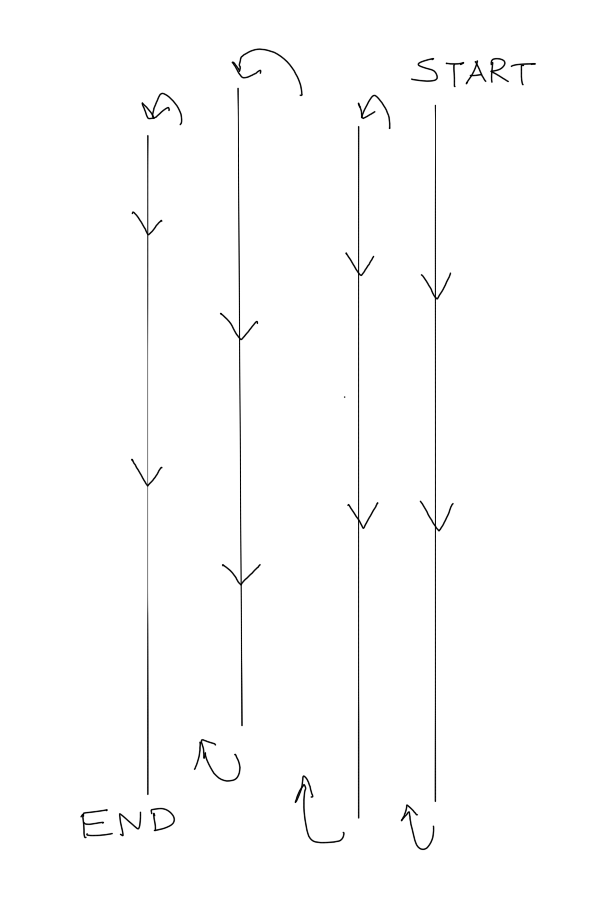
\includegraphics{stems}
\end{minipage}


\vfill

\begin{minipage}{0.45\textwidth}
     \centering
    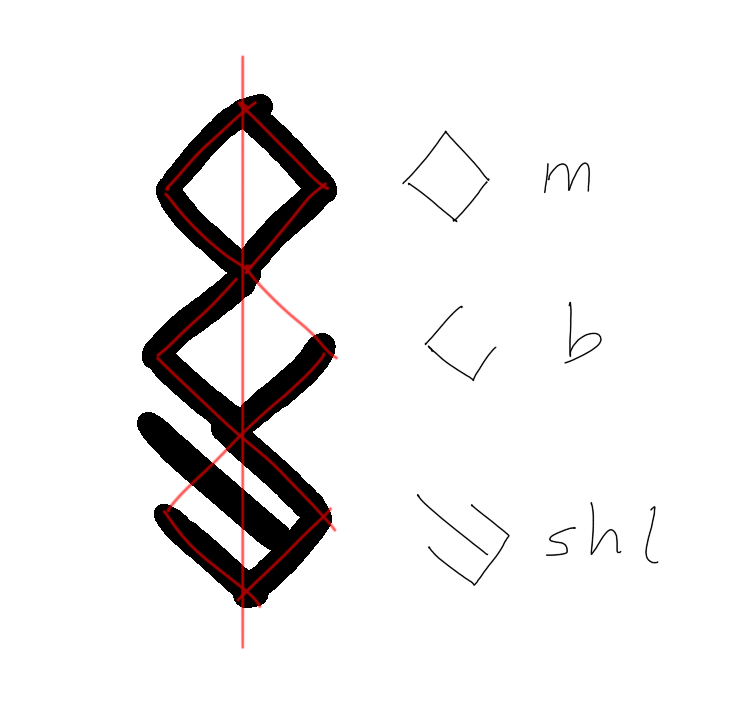
\includegraphics{mabashl}
\end{minipage}
\hfill
\begin{minipage}{0.5\textwidth}
The stem is included literally in some adults, so that words can appear as single connected shapes spanning vertically. Other adults break the stem line, so a disconnected symbol does \textbf{not} mean a word boundary. 

The adults themselves are all built, fundamentally, on a ``template'' of a 45\degree-rotated square, at least in the basic ``geometric'' style. The resulting visual coherence helps in distinguishing glyphs: each square is an adult. For example, the (imaginary) word \textbf{mabashl}, with adults \textbf{m}, \textbf{b}, \textbf{shl} becomes as on the left.

\end{minipage}

\vfill

\begin{minipage}[]{0.5\textwidth}
    Some rules are meant to be broken. Some really aren't. You can for example break free of the grid's vertical constraints. In the right example, the (again imaginary) word \textbf{damard} was stylized by stretching the vertical letter \textbf{d}; this is ok because this glyph, while meant to fit in a template square, does not really follow the lines of the square at all. Moreover, the two lower squares have been stretched into rhombi, and some curvature has been added to the lines. However, both rhombi are equal (approximately) in width and height. In general, stylization (at least for the Demorog script) can result in deformation of the fundamental square shape and stretching of non-square elements, but whenever the deformed squares appear, they should be consistent. This is essential for distinguishing adult boundaries (is there a joke here?).
\end{minipage}
\hfill
\begin{minipage}{0.45\textwidth}
    \centering
    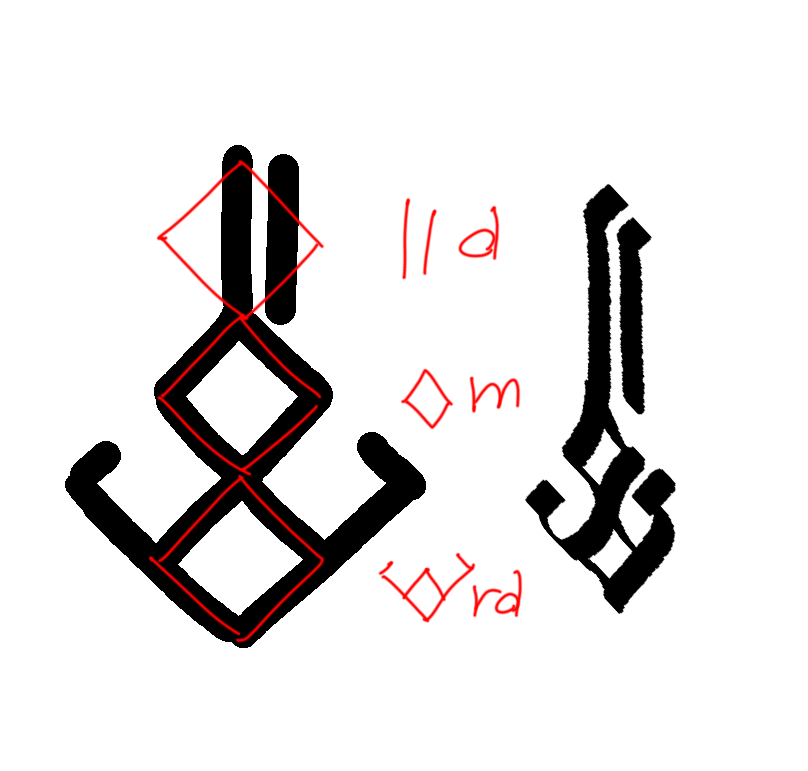
\includegraphics{damard}
\end{minipage}

\vfill

\pagebreak


\section{Children}

\begin{center}
    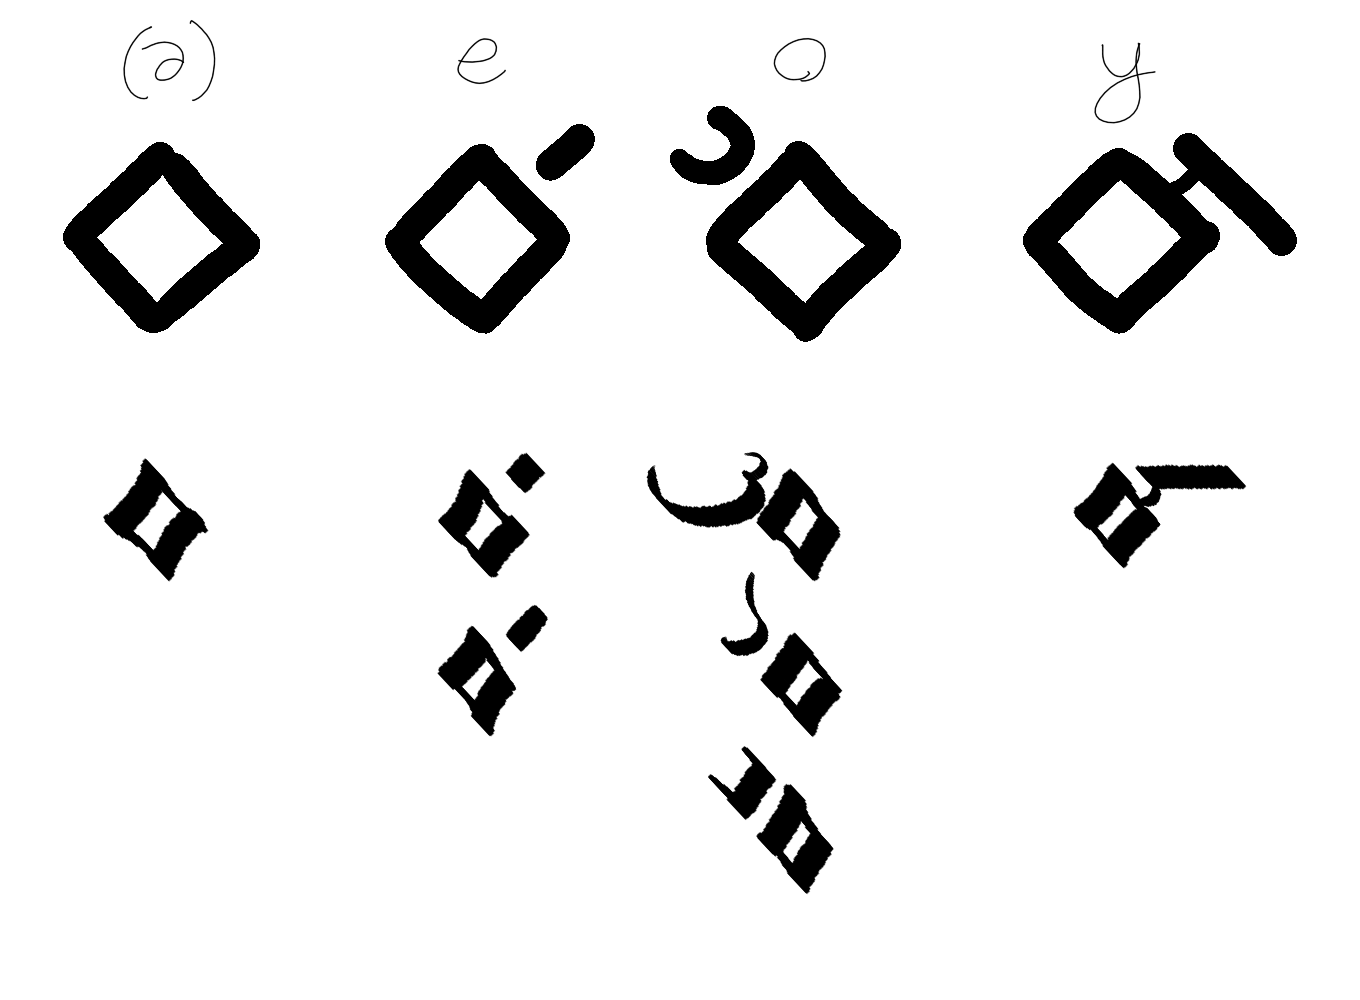
\includegraphics{childrenguide}
\end{center}

The four children markings (the absence of a marking is also considered a vowel letter by Flavans) are depicted here on the letter \textbf{m}. Below, a few variants for the cursive style are presented. There is great freedom in stylization of position and shape of vowel markings, because there is little chance of ambiguity; this freedom should be employed to avoid overlap of the markings with the previous adult. Some guidelines should be however satisfied to guarantee legibility:

\begin{itemize}
    \item \textbf{e} should always be detached from all adults and children on the same column and to the right of its parent adult, \textbf{upper} right if the adult includes a guide square. It should be either dot-like or angle upwards going to the right. It should be straight.
    \item \textbf{o} should also be detached from all glyphs of the column and on the left or upper left of its adult. It can take a great variety of shapes, generally c-like curves with the opening to the upper left, and might include one, two, or even three arcs. On many adults, however, the \textbf{o} and the adult join to create another form (generally it turns into a ``hook'' for the adult), the full syllabary table includes all possible combinations.
    \item \textbf{y} is attached by a little stem to its parent adult. Otherwise, it should not attach to anything else in the same column. The point of attachement is specific to each letter (see the full syllabary table) but it's always either right or upper right. The main stroke angles downward in the strict geometric style but is horizontal in handwritten geometric or in cursive.
\end{itemize}





\section{Syllabary (Males)}
The following are adult-child combination for the ``common'' adults, the ``males'', in geometric style. Some non-obvious cursive version of the geometric glyphs are depicted to their lower-right. The combination \textbf{ngy} contains in the cursive script the only permissible intersection of strokes. Note that the glyphs \textbf{g} and \textbf{s} interrupt the stem above, so there is a space between the adult and the one before. Similarly, \textbf{k} breaks below, and \textbf{t} breaks both above and below.

\begin{center}
    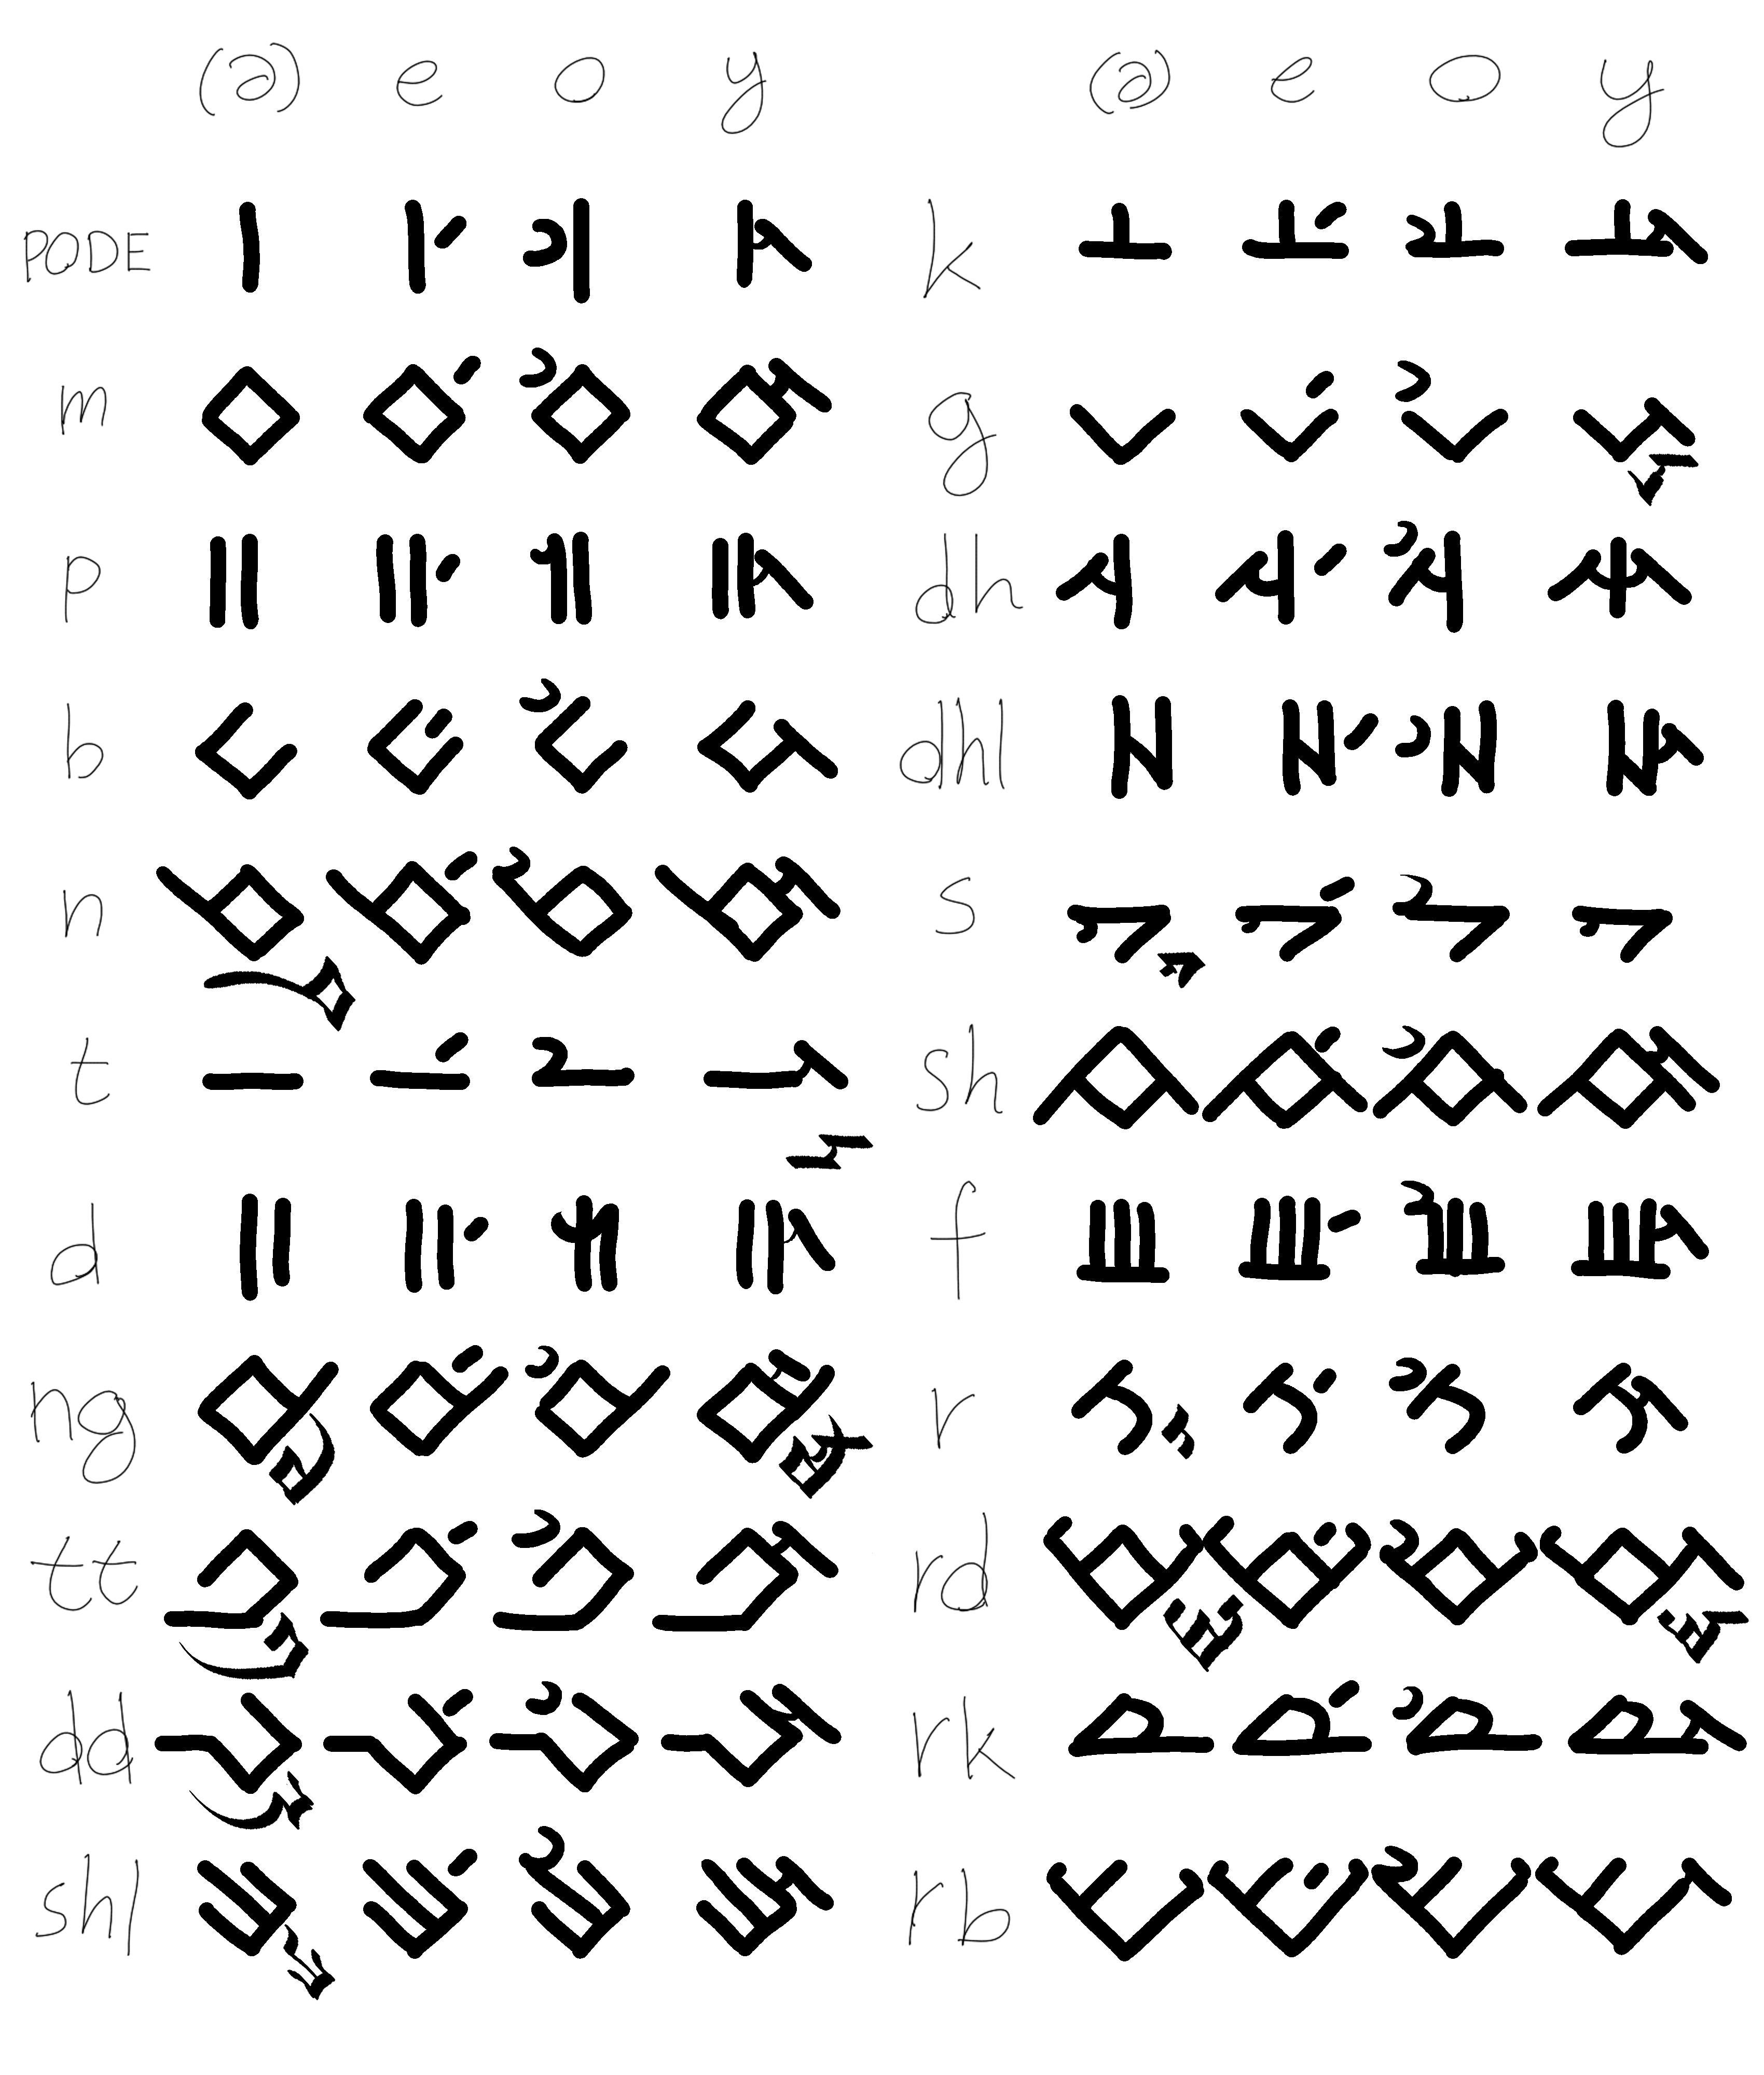
\includegraphics[scale=0.60]{syllabary_males}
\end{center}


%\pagebreak

\begin{samepage}

\section{Syllabary (Females)}
    And here are the more ``uncommon'' glyphs, the ``females''. \textbf{ttk} and \textbf{ttg} are identical; the only distinguishing feature is that the former does not interrupt the main stem while the latter does (and there's a corresponding space before the next letter). The very rare \textbf{pd} glyph must necessarily be drawn bigger than a square in the cursive script for the strokes to be distinct.
\
\begin{center}
    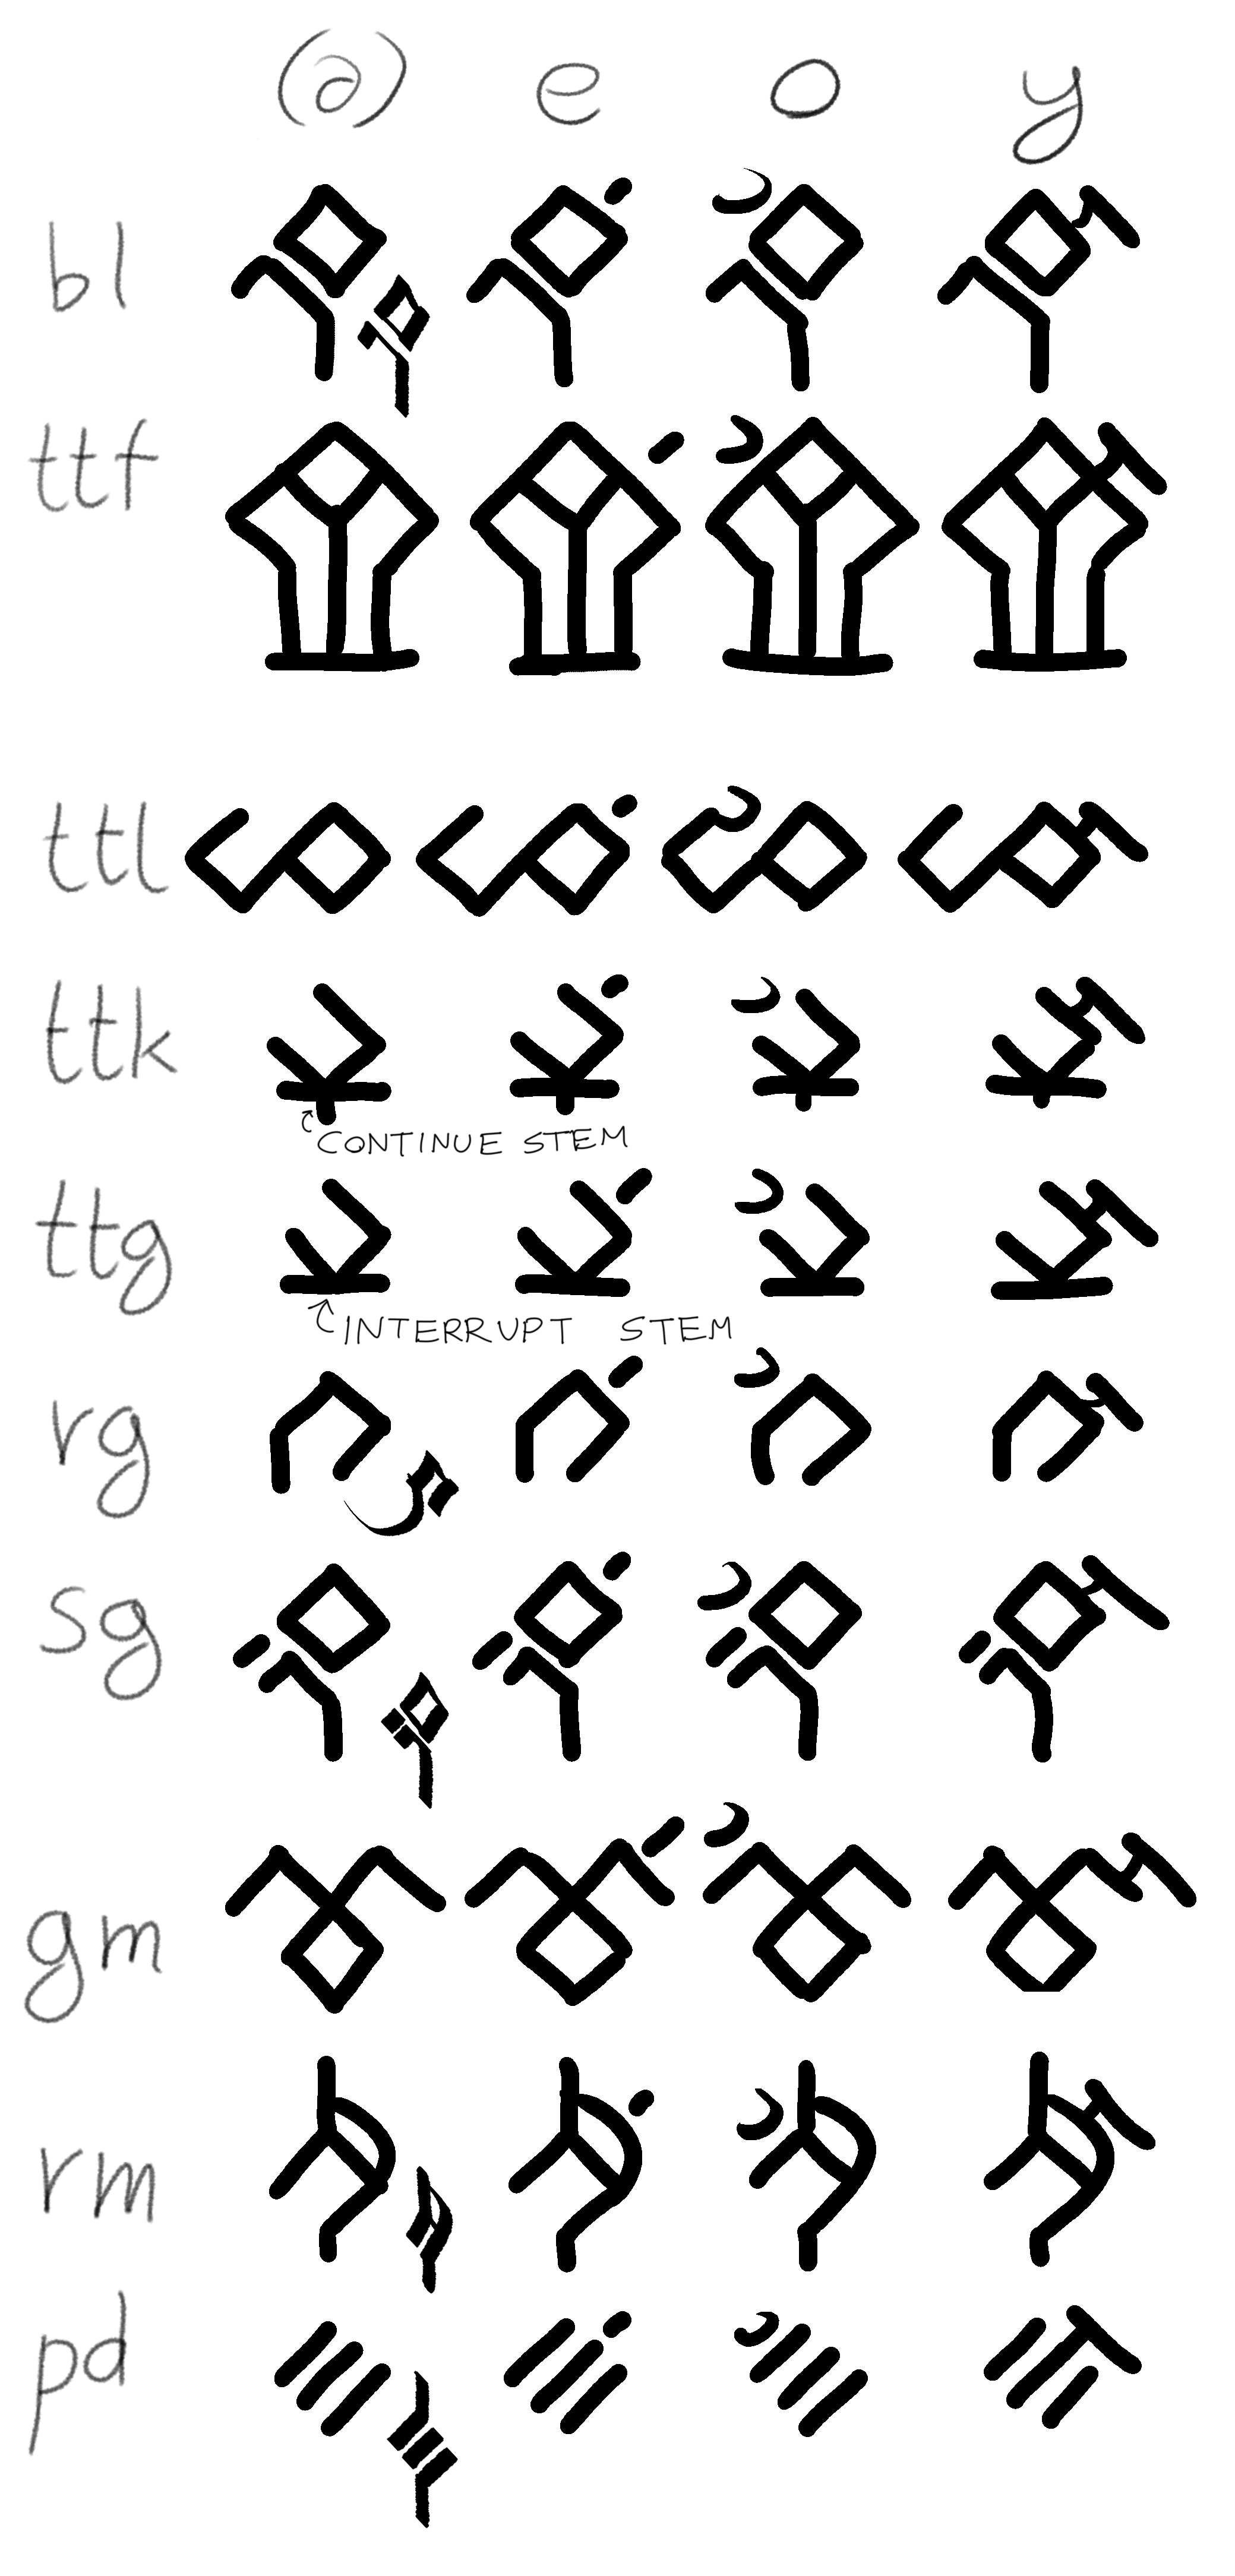
\includegraphics[scale=0.60]{syllabary_females}
\end{center}

\end{samepage}

\pagebreak




\section{Orthography and punctuation}

\vfill

\begin{minipage}[]{0.5\textwidth}
    There's one last ``letter'' to add: by reducing the space between consecutive \textbf{k} and \textbf{t} letters, one obtains a glyph for \textbf{kt}, representing the sound \apa{kt}. This can only be word-final and it's generally a consequence of a genitive ending where the last vowel has disappeared. In the rare case that a word does literally end in \textbf{kat}, an extra amount of space has to be introduced to clarify this.
\end{minipage}
\hfill
\begin{minipage}[]{0.45 \textwidth}
    \centering
    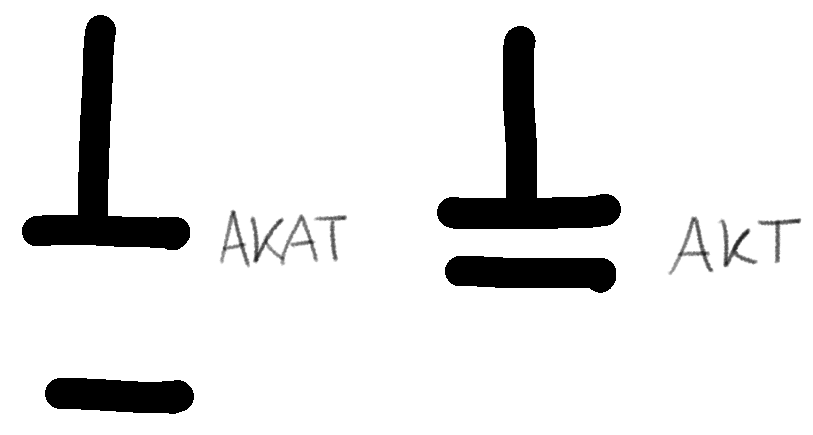
\includegraphics{kt}
\end{minipage}

\vfill

\begin{minipage}[]{0.45\textwidth}
    \centering
    
\includegraphics{ngonsettakad}
\end{minipage}
\hfill
\begin{minipage}[]{0.5\textwidth}
    Dots (or small strokes) aligned with the stem line separate words. They are identical to the \textbf{e} marking except for the positioning, in all styles. Words \textbf{never} span multiple columns, and no marking is placed when the column ends.

    Note that Flavans might separate words differently than the standard employed romanization, and that there are numerous irregularities and regional variants to this.
\end{minipage}

\vfill
\vspace{-50pt}

\begin{minipage}[]{0.5\textwidth}
    Three dots in a triangle mark the beginning of a quote, song, or direct speech. Two dots are sometimes (but not often, and surely not consistently) used to separate long periods or sentences. Three dots in text mark that the following is a name (signature, author, reference).
\end{minipage}
\hfill
\begin{minipage}[]{0.45\textwidth}
    \centering
    
\includegraphics{piss}
\end{minipage}

\vfill


\vspace{-50pt}

\begin{minipage}[]{0.45\textwidth}
    \centering
    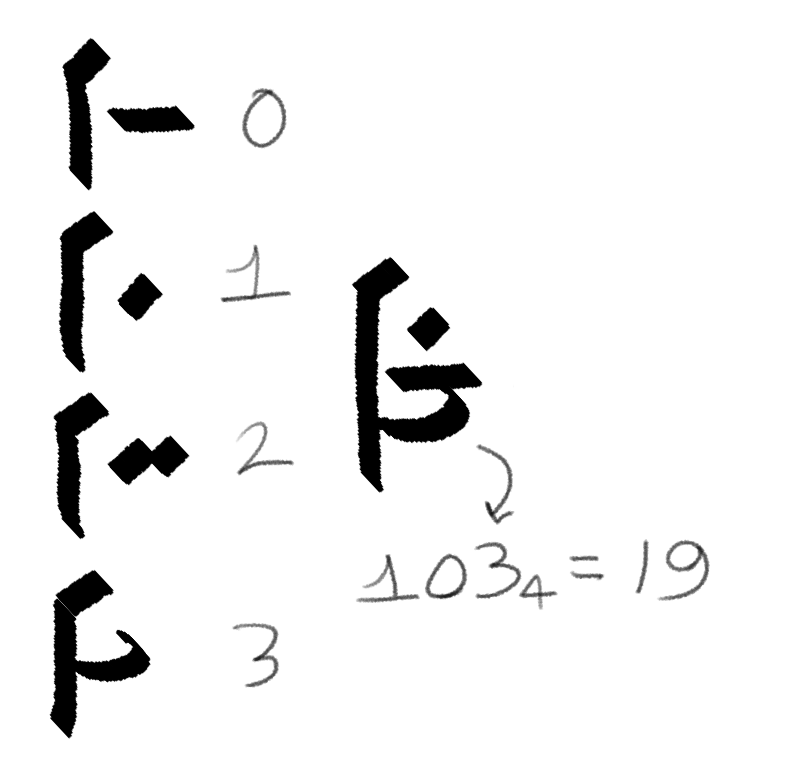
\includegraphics{digits}
\end{minipage}
\hfill
\begin{minipage}[]{0.5\textwidth}
    Flavans, after way more careful deliberation than was honestly necessary, have settled on a positional system for writing numbers, the \textbf{Borg system}. To write a number, draw a pode, then draw its digits in base $4$ from top to bottom using the scheme to the left.
\end{minipage}



\vfill

\pagebreak

\section{Font test}

{\Large
    \begin{tabular}[]{*{5}{c|}}
        \flav{ma} &\flav{me} &\flav{my} &\flav{mo} &\\\flav{na} &\flav{ne} &\flav{ny} &\flav{no} &\\\flav{ka} &\flav{ke} &\flav{ky} &\flav{ko} &\\\flav{ta} &\flav{te} &\flav{ty} &\flav{to} &\\\flav{da} &\flav{de} &\flav{dy} &\flav{do} &\\\flav{ga} &\flav{ge} &\flav{gy} &\flav{go} &\\\flav{ra} &\flav{re} &\flav{ry} &\flav{ro} &\\\flav{nga} &\flav{nge} &\flav{ngy} &\flav{ngo} &\\\flav{sa} &\flav{se} &\flav{sy} &\flav{so} &\\\flav{la} &\flav{le} &\flav{ly} &\flav{lo} &\\\flav{shla} &\flav{shle} &\flav{shly} &\flav{shlo} &\\\flav{dha} &\flav{dhe} &\flav{dhy} &\flav{dho} &\\\flav{dhla} &\flav{dhle} &\flav{dhly} &\flav{dhlo} &\\\flav{pa} &\flav{pe} &\flav{py} &\flav{po} &\\\flav{ba} &\flav{be} &\flav{by} &\flav{bo} &\\\flav{rda} &\flav{rde} &\flav{rdy} &\flav{rdo} &\\\flav{rba} &\flav{rbe} &\flav{rby} &\flav{rbo} &\\\flav{fa} &\flav{fe} &\flav{fy} &\flav{fo} &\\\flav{sha} &\flav{she} &\flav{shy} &\flav{sho} &\\\flav{tta} &\flav{tte} &\flav{tty} &\flav{tto} &\\\flav{dda} &\flav{dde} &\flav{ddy} &\flav{ddo} &\\\flav{rka} &\flav{rke} &\flav{rky} &\flav{rko} &\\\flav{ttla} &\flav{ttle} &\flav{ttly} &\flav{ttlo} &\\\flav{dda} &\flav{dde} &\flav{ddy} &\flav{ddo} &\\\flav{ttka} &\flav{ttke} &\flav{ttky} &\flav{ttko} &\\\flav{rga} &\flav{rge} &\flav{rgy} &\flav{rgo} &\\\flav{gma} &\flav{gme} &\flav{gmy} &\flav{gmo} &\\\flav{pda} &\flav{pde} &\flav{pdy} &\flav{pdo} &\\\flav{bla} &\flav{ble} &\flav{bly} &\flav{blo} &\\\flav{ttfa} &\flav{ttfe} &\flav{ttfy} &\flav{ttfo} &\\\flav{sga} &\flav{sge} &\flav{sgy} &\flav{sgo} &\\\flav{ttga} &\flav{ttge} &\flav{ttgy} &\flav{ttgo} &\\
    \end{tabular}

}

\end{document}
